% $Header: /u/gcmpack/manual/s_software/text/sarch.tex,v 1.24 2006/04/05 01:12:02 jmc Exp $

This chapter focuses on describing the {\bf WRAPPER} environment
within which both the core numerics and the pluggable packages
operate. The description presented here is intended to be a detailed
exposition and contains significant background material, as well as
advanced details on working with the WRAPPER.  The tutorial sections
of this manual (see sections \ref{sect:tutorials} and
\ref{sect:tutorialIII}) contain more succinct, step-by-step
instructions on running basic numerical experiments, of varous types,
both sequentially and in parallel. For many projects simply starting
from an example code and adapting it to suit a particular situation
will be all that is required.  The first part of this chapter
discusses the MITgcm architecture at an abstract level. In the second
part of the chapter we described practical details of the MITgcm
implementation and of current tools and operating system features that
are employed.

\section{Overall architectural goals}
\begin{rawhtml}
<!-- CMIREDIR:overall_architectural_goals: -->
\end{rawhtml}

Broadly, the goals of the software architecture employed in MITgcm are 
three-fold
 
\begin{itemize}
\item We wish to be able to study a very broad range of interesting
  and challenging rotating fluids problems.
\item We wish the model code to be readily targeted to a wide range of
  platforms
\item On any given platform we would like to be able to achieve
  performance comparable to an implementation developed and
  specialized specifically for that platform.
\end{itemize}

These points are summarized in figure
\ref{fig:mitgcm_architecture_goals} which conveys the goals of the
MITgcm design. The goals lead to a software architecture which at the
high-level can be viewed as consisting of

\begin{enumerate}
\item A core set of numerical and support code. This is discussed in
  detail in section \ref{chap:discretization}.

\item A scheme for supporting optional ``pluggable'' {\bf packages}
  (containing for example mixed-layer schemes, biogeochemical schemes,
  atmospheric physics).  These packages are used both to overlay
  alternate dynamics and to introduce specialized physical content
  onto the core numerical code. An overview of the {\bf package}
  scheme is given at the start of part \ref{chap:packagesI}.

\item A support framework called {\bf WRAPPER} (Wrappable Application
  Parallel Programming Environment Resource), within which the core
  numerics and pluggable packages operate.
\end{enumerate}

This chapter focuses on describing the {\bf WRAPPER} environment under
which both the core numerics and the pluggable packages function. The
description presented here is intended to be a detailed exposition and
contains significant background material, as well as advanced details
on working with the WRAPPER.  The examples section of this manual
(part \ref{chap:getting_started}) contains more succinct, step-by-step
instructions on running basic numerical experiments both sequentially
and in parallel. For many projects simply starting from an example
code and adapting it to suit a particular situation will be all that
is required.


\begin{figure}
\begin{center}
\resizebox{!}{2.5in}{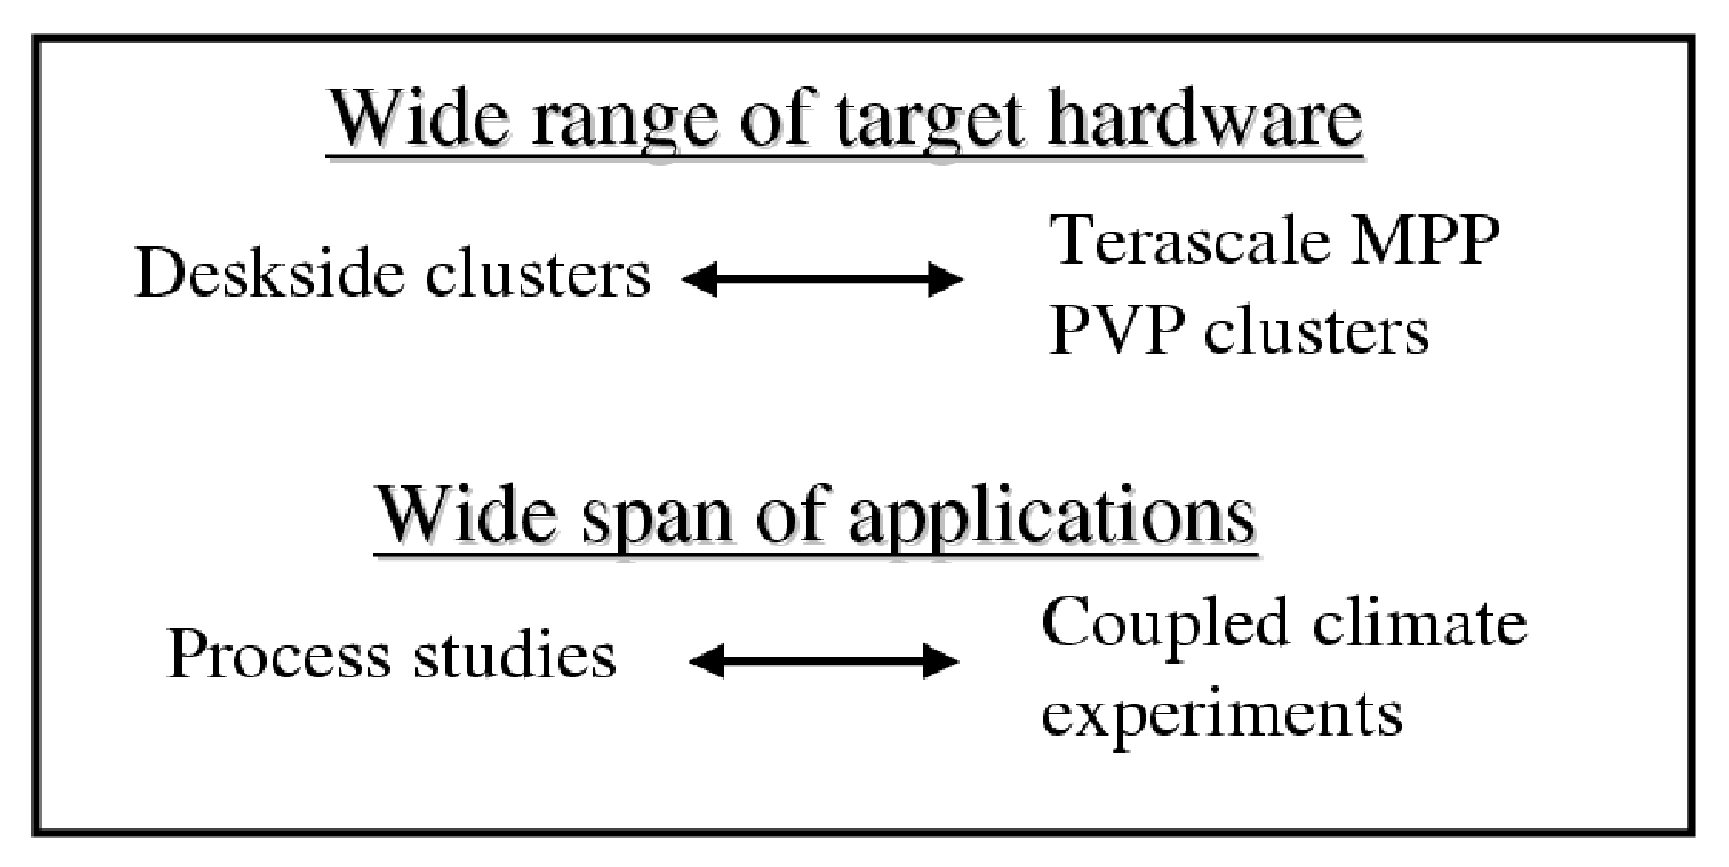
\includegraphics{part4/mitgcm_goals.eps}}
\end{center}
\caption{ The MITgcm architecture is designed to allow simulation of a
  wide range of physical problems on a wide range of hardware. The
  computational resource requirements of the applications targeted
  range from around $10^7$ bytes ($\approx 10$ megabytes) of memory to
  $10^{11}$ bytes ($\approx 100$ gigabytes). Arithmetic operation
  counts for the applications of interest range from $10^{9}$ floating
  point operations to more than $10^{17}$ floating point operations.}
\label{fig:mitgcm_architecture_goals}
\end{figure}

\section{WRAPPER}
\begin{rawhtml}
<!-- CMIREDIR:wrapper: -->
\end{rawhtml}

A significant element of the software architecture utilized in MITgcm
is a software superstructure and substructure collectively called the
WRAPPER (Wrappable Application Parallel Programming Environment
Resource). All numerical and support code in MITgcm is written to
``fit'' within the WRAPPER infrastructure. Writing code to ``fit''
within the WRAPPER means that coding has to follow certain, relatively
straightforward, rules and conventions (these are discussed further in
section \ref{sect:specifying_a_decomposition}).

The approach taken by the WRAPPER is illustrated in figure
\ref{fig:fit_in_wrapper} which shows how the WRAPPER serves to
insulate code that fits within it from architectural differences
between hardware platforms and operating systems. This allows
numerical code to be easily retargetted.


\begin{figure}
\begin{center}
\resizebox{!}{4.5in}{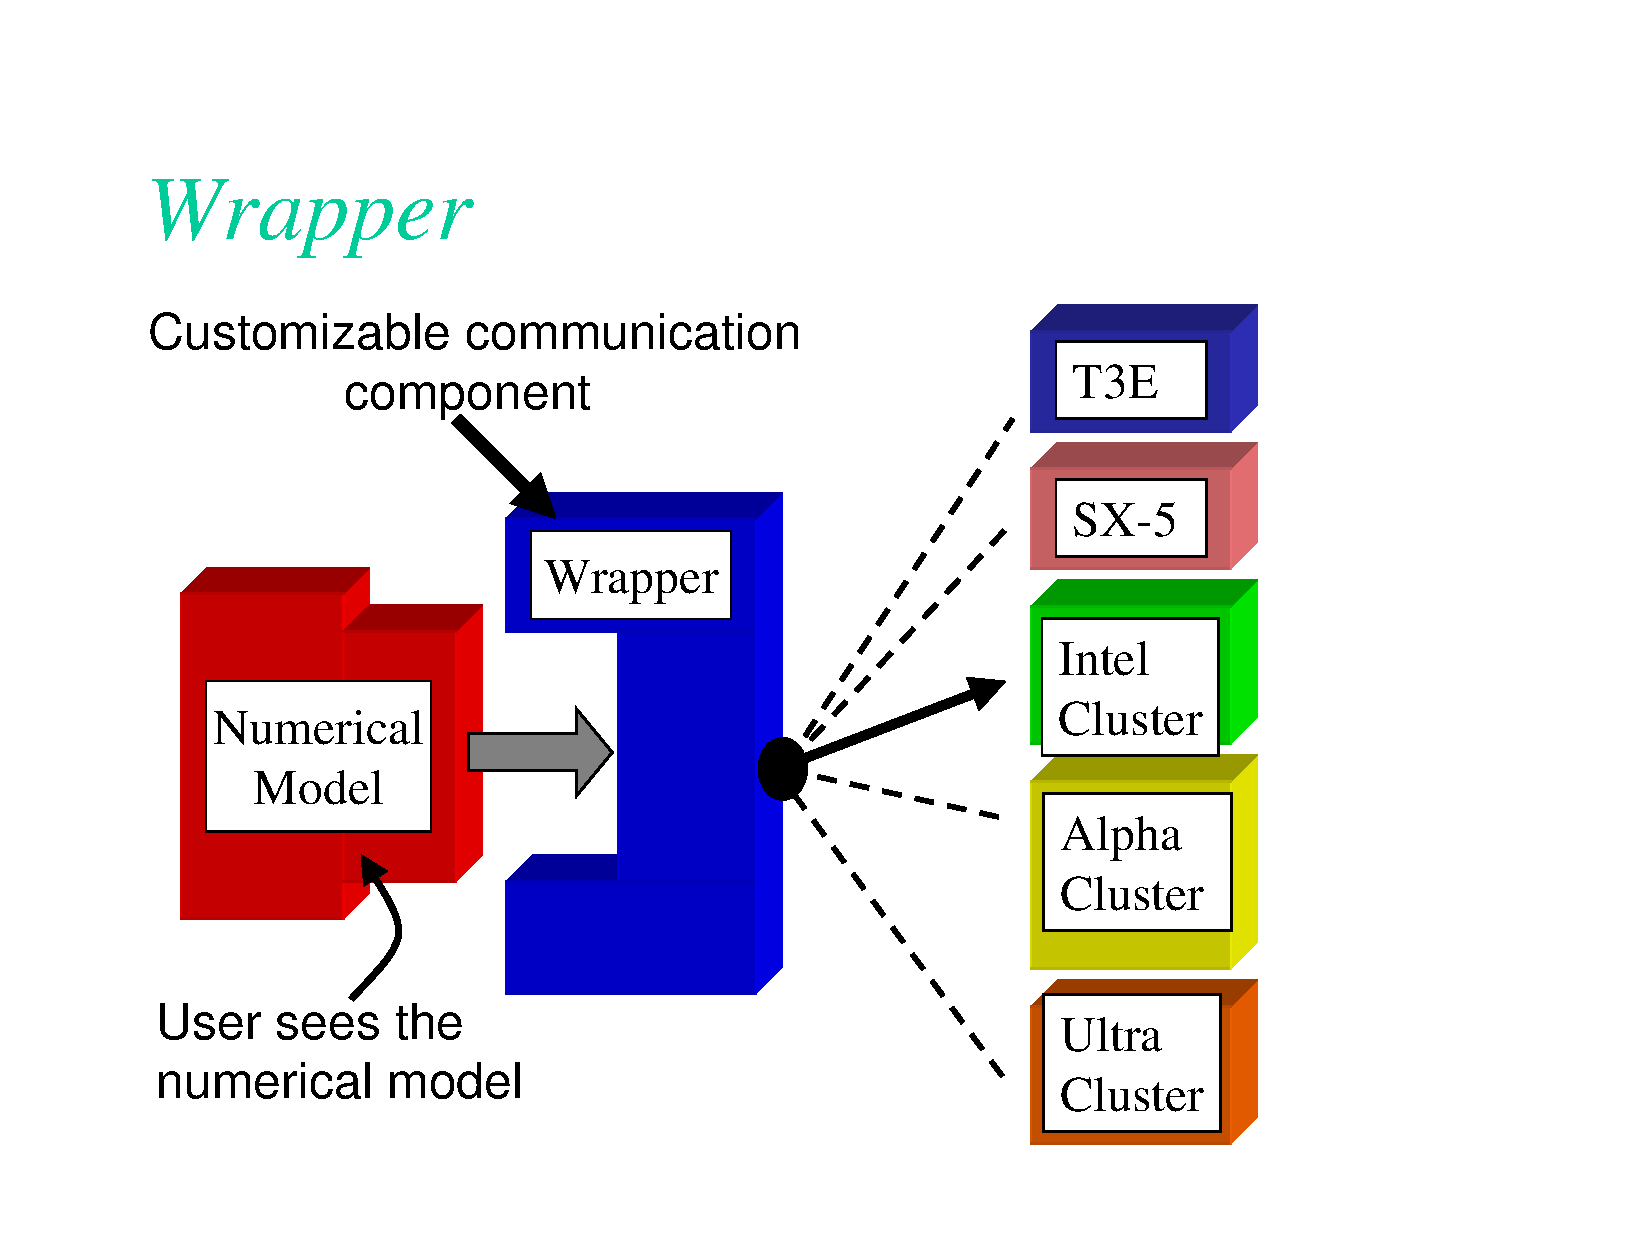
\includegraphics{part4/fit_in_wrapper.eps}}
\end{center}
\caption{
Numerical code is written to fit within a software support
infrastructure called WRAPPER. The WRAPPER is portable and
can be specialized for a wide range of specific target hardware and 
programming environments, without impacting numerical code that fits
within the WRAPPER. Codes that fit within the WRAPPER can generally be
made to run as fast on a particular platform as codes specially 
optimized for that platform.}
\label{fig:fit_in_wrapper}
\end{figure}

\subsection{Target hardware}
\label{sect:target_hardware}

The WRAPPER is designed to target as broad as possible a range of
computer systems.  The original development of the WRAPPER took place
on a multi-processor, CRAY Y-MP system. On that system, numerical code
performance and scaling under the WRAPPER was in excess of that of an
implementation that was tightly bound to the CRAY systems proprietary
multi-tasking and micro-tasking approach. Later developments have been
carried out on uniprocessor and multi-processor Sun systems with both
uniform memory access (UMA) and non-uniform memory access (NUMA)
designs.  Significant work has also been undertaken on x86 cluster
systems, Alpha processor based clustered SMP systems, and on
cache-coherent NUMA (CC-NUMA) systems such as Silicon Graphics Altix
systems.  The MITgcm code, operating within the WRAPPER, is also
routinely used on large scale MPP systems (for example, Cray T3E and
IBM SP systems). In all cases numerical code, operating within the
WRAPPER, performs and scales very competitively with equivalent
numerical code that has been modified to contain native optimizations
for a particular system \ref{ref hoe and hill, ecmwf}.

\subsection{Supporting hardware neutrality}

The different systems listed in section \ref{sect:target_hardware} can
be categorized in many different ways. For example, one common
distinction is between shared-memory parallel systems (SMP and PVP)
and distributed memory parallel systems (for example x86 clusters and
large MPP systems). This is one example of a difference between
compute platforms that can impact an application. Another common
distinction is between vector processing systems with highly
specialized CPUs and memory subsystems and commodity microprocessor
based systems. There are numerous other differences, especially in
relation to how parallel execution is supported. To capture the
essential differences between different platforms the WRAPPER uses a
{\it machine model}.

\subsection{WRAPPER machine model}

Applications using the WRAPPER are not written to target just one
particular machine (for example an IBM SP2) or just one particular
family or class of machines (for example Parallel Vector Processor
Systems). Instead the WRAPPER provides applications with an abstract
{\it machine model}. The machine model is very general, however, it
can easily be specialized to fit, in a computationally efficient
manner, any computer architecture currently available to the
scientific computing community.

\subsection{Machine model parallelism}
\label{sect:domain_decomposition}
\begin{rawhtml}
<!-- CMIREDIR:domain_decomp: -->
\end{rawhtml}

Codes operating under the WRAPPER target an abstract machine that is
assumed to consist of one or more logical processors that can compute
concurrently.  Computational work is divided among the logical
processors by allocating ``ownership'' to each processor of a certain
set (or sets) of calculations. Each set of calculations owned by a
particular processor is associated with a specific region of the
physical space that is being simulated, only one processor will be
associated with each such region (domain decomposition).

In a strict sense the logical processors over which work is divided do
not need to correspond to physical processors.  It is perfectly
possible to execute a configuration decomposed for multiple logical
processors on a single physical processor.  This helps ensure that
numerical code that is written to fit within the WRAPPER will
parallelize with no additional effort.  It is also useful for
debugging purposes.  Generally, however, the computational domain will
be subdivided over multiple logical processors in order to then bind
those logical processors to physical processor resources that can
compute in parallel.

\subsubsection{Tiles}

Computationally, the data structures (\textit{eg.} arrays, scalar
variables, etc.) that hold the simulated state are associated with
each region of physical space and are allocated to a particular
logical processor.  We refer to these data structures as being {\bf
  owned} by the processor to which their associated region of physical
space has been allocated.  Individual regions that are allocated to
processors are called {\bf tiles}.  A processor can own more than one
tile.  Figure \ref{fig:domaindecomp} shows a physical domain being
mapped to a set of logical processors, with each processors owning a
single region of the domain (a single tile).  Except for periods of
communication and coordination, each processor computes autonomously,
working only with data from the tile (or tiles) that the processor
owns.  When multiple tiles are alloted to a single processor, each
tile is computed on independently of the other tiles, in a sequential
fashion.

\begin{figure}
\begin{center}
 \resizebox{5in}{!}{
  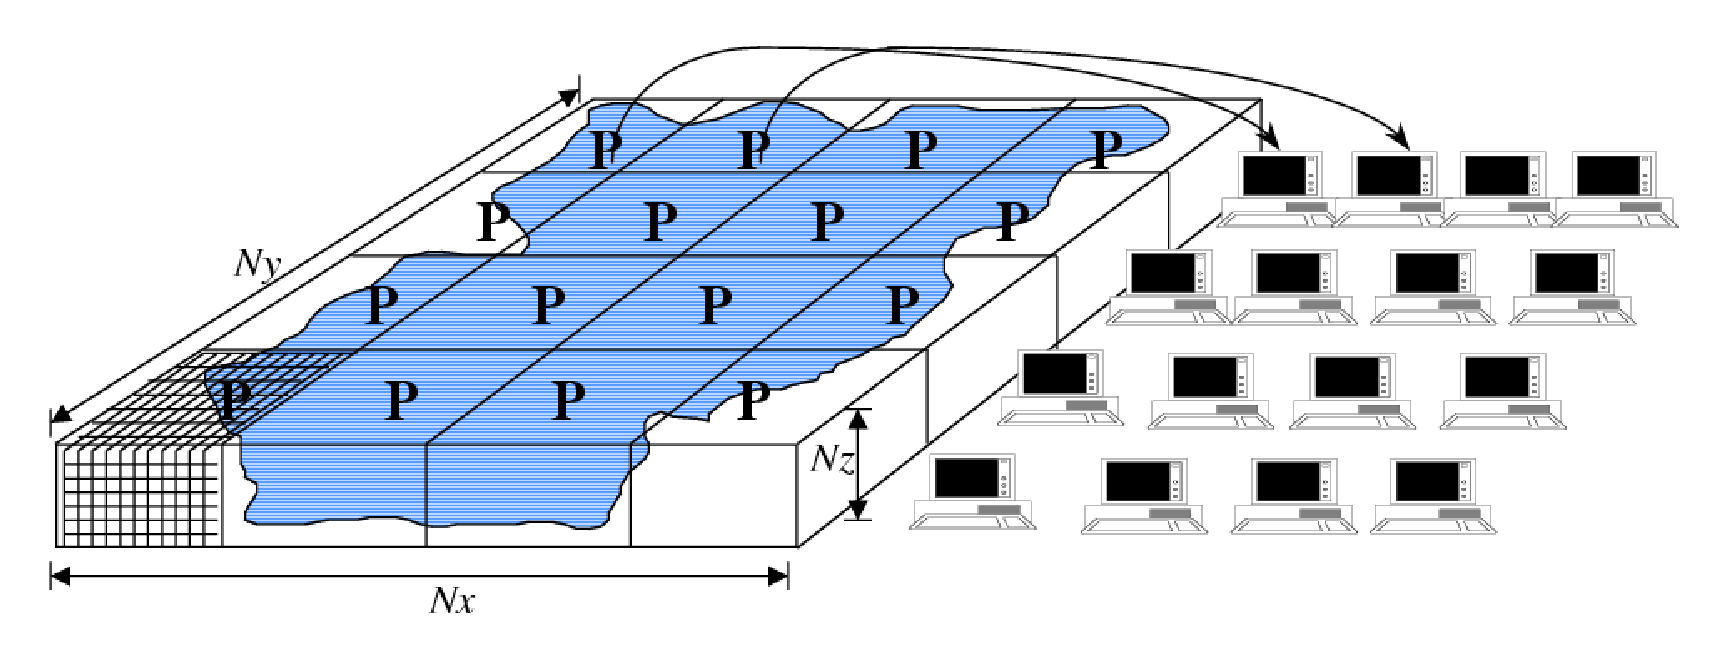
\includegraphics{part4/domain_decomp.eps}
 }
\end{center}
\caption{ The WRAPPER provides support for one and two dimensional
  decompositions of grid-point domains. The figure shows a
  hypothetical domain of total size $N_{x}N_{y}N_{z}$. This
  hypothetical domain is decomposed in two-dimensions along the
  $N_{x}$ and $N_{y}$ directions. The resulting {\bf tiles} are {\bf
    owned} by different processors. The {\bf owning} processors
  perform the arithmetic operations associated with a {\bf tile}.
  Although not illustrated here, a single processor can {\bf own}
  several {\bf tiles}.  Whenever a processor wishes to transfer data
  between tiles or communicate with other processors it calls a
  WRAPPER supplied function.  } \label{fig:domaindecomp}
\end{figure}


\subsubsection{Tile layout}

Tiles consist of an interior region and an overlap region.  The
overlap region of a tile corresponds to the interior region of an
adjacent tile.  In figure \ref{fig:tiledworld} each tile would own the
region within the black square and hold duplicate information for
overlap regions extending into the tiles to the north, south, east and
west.  During computational phases a processor will reference data in
an overlap region whenever it requires values that lie outside the
domain it owns.  Periodically processors will make calls to WRAPPER
functions to communicate data between tiles, in order to keep the
overlap regions up to date (see section
\ref{sect:communication_primitives}).  The WRAPPER functions can use a
variety of different mechanisms to communicate data between tiles.

\begin{figure}
\begin{center}
 \resizebox{5in}{!}{
  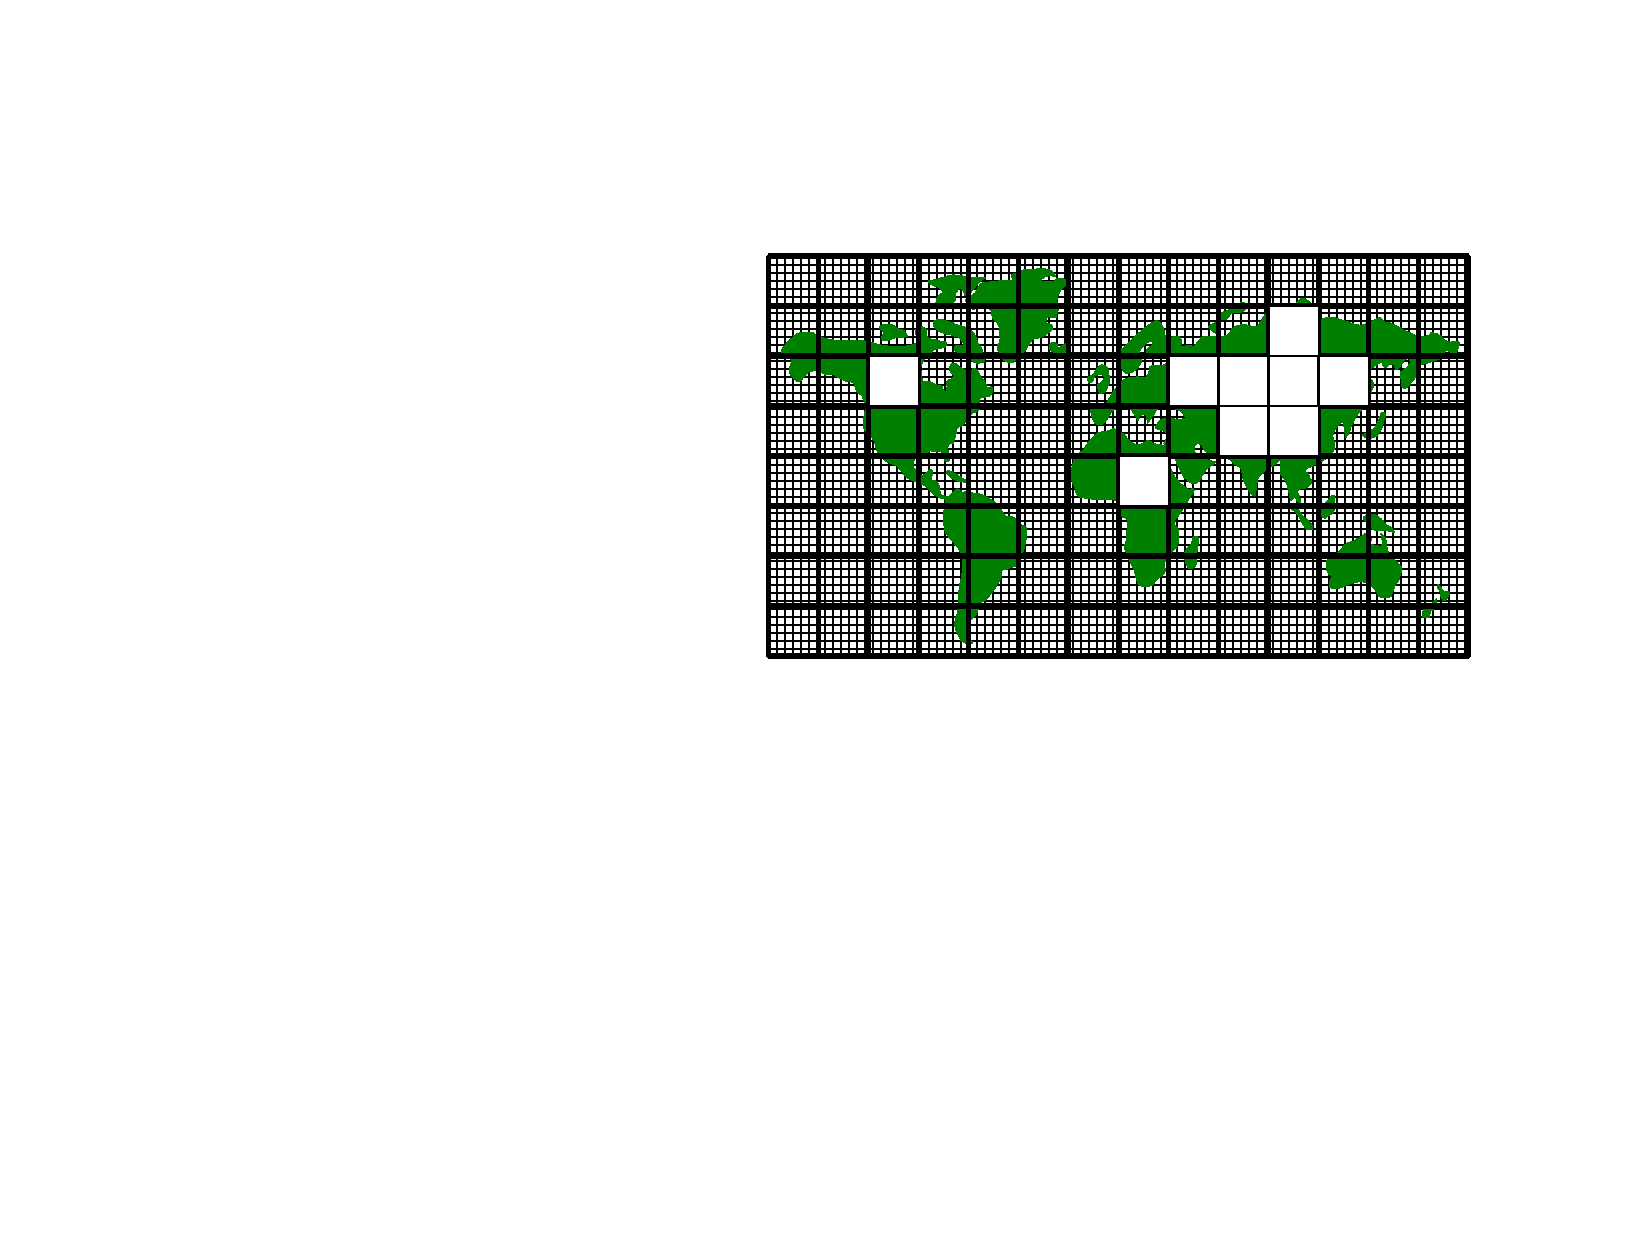
\includegraphics{part4/tiled-world.eps}
 }
\end{center}
\caption{ A global grid subdivided into tiles.
Tiles contain a interior region and an overlap region.
Overlap regions are periodically updated from neighboring tiles.
} \label{fig:tiledworld} 
\end{figure}

\subsection{Communication mechanisms}

Logical processors are assumed to be able to exchange information
between tiles and between each other using at least one of two
possible mechanisms.

\begin{itemize}
\item {\bf Shared memory communication}.  Under this mode of
  communication data transfers are assumed to be possible using direct
  addressing of regions of memory.  In this case a CPU is able to read
  (and write) directly to regions of memory ``owned'' by another CPU
  using simple programming language level assignment operations of the
  the sort shown in figure \ref{fig:simple_assign}.  In this way one
  CPU (CPU1 in the figure) can communicate information to another CPU
  (CPU2 in the figure) by assigning a particular value to a particular
  memory location.

\item {\bf Distributed memory communication}.  Under this mode of
  communication there is no mechanism, at the application code level,
  for directly addressing regions of memory owned and visible to
  another CPU. Instead a communication library must be used as
  illustrated in figure \ref{fig:comm_msg}. In this case CPUs must
  call a function in the API of the communication library to
  communicate data from a tile that it owns to a tile that another CPU
  owns. By default the WRAPPER binds to the MPI communication library
  \ref{MPI} for this style of communication.
\end{itemize}

The WRAPPER assumes that communication will use one of these two styles
of communication.  The underlying hardware and operating system support
for the style used is not specified and can vary from system to system.

\begin{figure}
\begin{verbatim}

         CPU1                    |        CPU2
         ====                    |        ====
                                 |
       a(3) = 8                  |        WHILE ( a(3) .NE. 8 ) 
                                 |         WAIT
                                 |        END WHILE
                                 |
\end{verbatim}
\caption{In the WRAPPER shared memory communication model, simple writes to an
array can be made to be visible to other CPUs at the application code level.
So that for example, if one CPU (CPU1 in the figure above) writes the value $8$ to 
element $3$ of array $a$, then other CPUs (for example CPU2 in the figure above)
will be able to see the value $8$ when they read from $a(3)$.
This provides a very low latency and high bandwidth communication 
mechanism.
} \label{fig:simple_assign}
\end{figure}

\begin{figure}
\begin{verbatim}

         CPU1                    |        CPU2
         ====                    |        ====
                                 |
       a(3) = 8                  |        WHILE ( a(3) .NE. 8 )
       CALL SEND( CPU2,a(3) )    |         CALL RECV( CPU1, a(3) )
                                 |        END WHILE
                                 |
\end{verbatim}
\caption{ In the WRAPPER distributed memory communication model
data can not be made directly visible to other CPUs.
If one CPU writes the value $8$ to element $3$ of array $a$, then
at least one of CPU1 and/or CPU2 in the figure above will need
to call a bespoke communication library in order for the updated 
value to be communicated between CPUs.
} \label{fig:comm_msg}
\end{figure}

\subsection{Shared memory communication}
\label{sect:shared_memory_communication}

Under shared communication independent CPUs are operating on the
exact same global address space at the application level.  This means
that CPU 1 can directly write into global data structures that CPU 2
``owns'' using a simple assignment at the application level.  This is
the model of memory access is supported at the basic system design
level in ``shared-memory'' systems such as PVP systems, SMP systems,
and on distributed shared memory systems (\textit{eg.} SGI Origin, SGI
Altix, and some AMD Opteron systems).  On such systems the WRAPPER
will generally use simple read and write statements to access directly
application data structures when communicating between CPUs.

In a system where assignments statements, like the one in figure
\ref{fig:simple_assign} map directly to hardware instructions that
transport data between CPU and memory banks, this can be a very
efficient mechanism for communication.  In this case two CPUs, CPU1
and CPU2, can communicate simply be reading and writing to an agreed
location and following a few basic rules.  The latency of this sort of
communication is generally not that much higher than the hardware
latency of other memory accesses on the system. The bandwidth
available between CPUs communicating in this way can be close to the
bandwidth of the systems main-memory interconnect.  This can make this
method of communication very efficient provided it is used
appropriately.

\subsubsection{Memory consistency}
\label{sect:memory_consistency}

When using shared memory communication between multiple processors the
WRAPPER level shields user applications from certain counter-intuitive
system behaviors.  In particular, one issue the WRAPPER layer must
deal with is a systems memory model.  In general the order of reads
and writes expressed by the textual order of an application code may
not be the ordering of instructions executed by the processor
performing the application.  The processor performing the application
instructions will always operate so that, for the application
instructions the processor is executing, any reordering is not
apparent.  However, in general machines are often designed so that
reordering of instructions is not hidden from other second processors.
This means that, in general, even on a shared memory system two
processors can observe inconsistent memory values.

The issue of memory consistency between multiple processors is
discussed at length in many computer science papers.  From a practical
point of view, in order to deal with this issue, shared memory
machines all provide some mechanism to enforce memory consistency when
it is needed.  The exact mechanism employed will vary between systems.
For communication using shared memory, the WRAPPER provides a place to
invoke the appropriate mechanism to ensure memory consistency for a
particular platform.

\subsubsection{Cache effects and false sharing}
\label{sect:cache_effects_and_false_sharing}

Shared-memory machines often have local to processor memory caches
which contain mirrored copies of main memory.  Automatic cache-coherence
protocols are used to maintain consistency between caches on different
processors.  These cache-coherence protocols typically enforce consistency
between regions of memory with large granularity (typically 128 or 256 byte
chunks).  The coherency protocols employed can be expensive relative to other
memory accesses and so care is taken in the WRAPPER (by padding synchronization
structures appropriately) to avoid unnecessary coherence traffic.

\subsubsection{Operating system support for shared memory.}

Applications running under multiple threads within a single process
can use shared memory communication.  In this case {\it all} the
memory locations in an application are potentially visible to all the
compute threads. Multiple threads operating within a single process is
the standard mechanism for supporting shared memory that the WRAPPER
utilizes. Configuring and launching code to run in multi-threaded mode
on specific platforms is discussed in section
\ref{sect:multi-threaded-execution}.  However, on many systems,
potentially very efficient mechanisms for using shared memory
communication between multiple processes (in contrast to multiple
threads within a single process) also exist. In most cases this works
by making a limited region of memory shared between processes. The
MMAP \ref{magicgarden} and IPC \ref{magicgarden} facilities in UNIX
systems provide this capability as do vendor specific tools like LAPI
\ref{IBMLAPI} and IMC \ref{Memorychannel}.  Extensions exist for the
WRAPPER that allow these mechanisms to be used for shared memory
communication. However, these mechanisms are not distributed with the
default WRAPPER sources, because of their proprietary nature.

\subsection{Distributed memory communication}
\label{sect:distributed_memory_communication}
Many parallel systems are not constructed in a way where it is
possible or practical for an application to use shared memory for
communication. For example cluster systems consist of individual
computers connected by a fast network. On such systems there is no
notion of shared memory at the system level. For this sort of system
the WRAPPER provides support for communication based on a bespoke
communication library (see figure \ref{fig:comm_msg}).  The default
communication library used is MPI \cite{MPI-std-20}. However, it is
relatively straightforward to implement bindings to optimized platform
specific communication libraries. For example the work described in
\ref{hoe-hill:99} substituted standard MPI communication for a highly
optimized library.

\subsection{Communication primitives}
\label{sect:communication_primitives}

\begin{figure}
\begin{center}
 \resizebox{5in}{!}{
  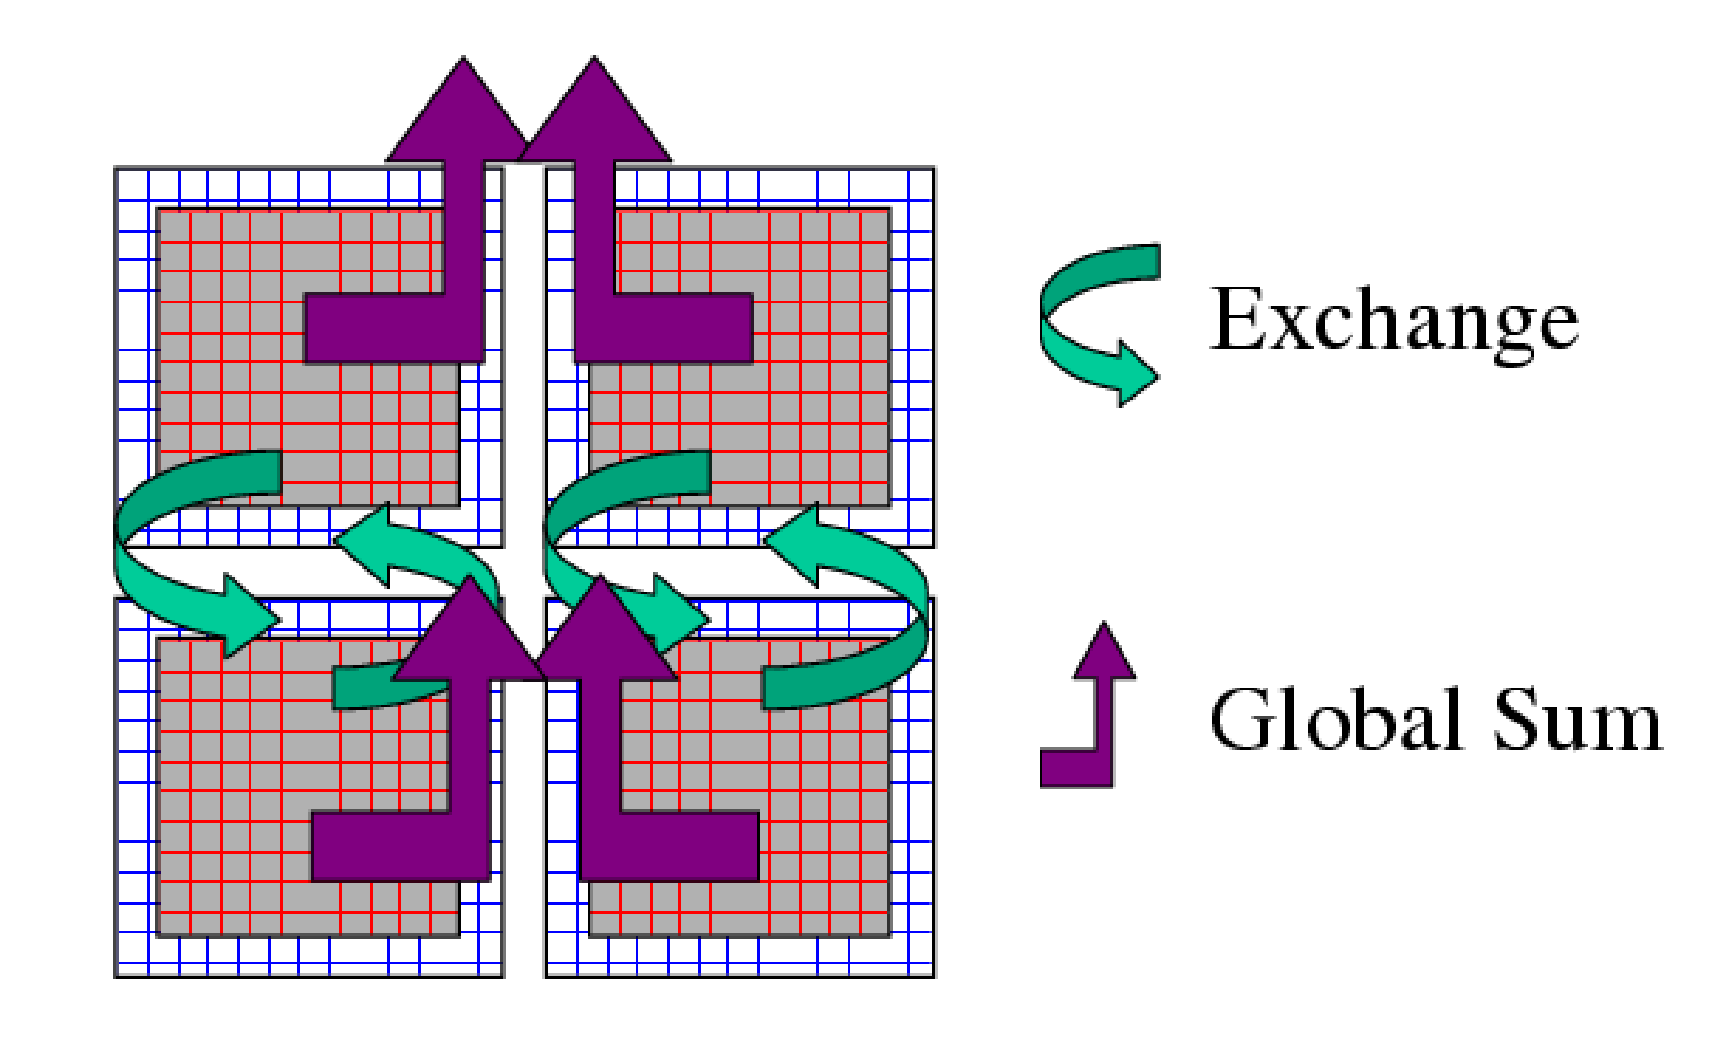
\includegraphics{part4/comm-primm.eps}
 }
\end{center}
\caption{Three performance critical parallel primitives are provided
  by the WRAPPER. These primitives are always used to communicate data
  between tiles. The figure shows four tiles. The curved arrows
  indicate exchange primitives which transfer data between the overlap
  regions at tile edges and interior regions for nearest-neighbor
  tiles.  The straight arrows symbolize global sum operations which
  connect all tiles.  The global sum operation provides both a key
  arithmetic primitive and can serve as a synchronization primitive. A
  third barrier primitive is also provided, it behaves much like the
  global sum primitive.  } \label{fig:communication_primitives}
\end{figure}


Optimized communication support is assumed to be potentially available
for a small number of communication operations.  It is also assumed
that communication performance optimizations can be achieved by
optimizing a small number of communication primitives.  Three
optimizable primitives are provided by the WRAPPER
\begin{itemize}
\item{\bf EXCHANGE} This operation is used to transfer data between
  interior and overlap regions of neighboring tiles. A number of
  different forms of this operation are supported. These different
  forms handle
  \begin{itemize}
  \item Data type differences. Sixty-four bit and thirty-two bit
    fields may be handled separately.
  \item Bindings to different communication methods.  Exchange
    primitives select between using shared memory or distributed
    memory communication.
  \item Transformation operations required when transporting data
    between different grid regions. Transferring data between faces of
    a cube-sphere grid, for example, involves a rotation of vector
    components.
  \item Forward and reverse mode computations. Derivative calculations
    require tangent linear and adjoint forms of the exchange
    primitives.
  \end{itemize}

\item{\bf GLOBAL SUM} The global sum operation is a central arithmetic
  operation for the pressure inversion phase of the MITgcm algorithm.
  For certain configurations scaling can be highly sensitive to the
  performance of the global sum primitive. This operation is a
  collective operation involving all tiles of the simulated domain.
  Different forms of the global sum primitive exist for handling
  \begin{itemize}
  \item Data type differences. Sixty-four bit and thirty-two bit
    fields may be handled separately.
  \item Bindings to different communication methods.  Exchange
    primitives select between using shared memory or distributed
    memory communication.
  \item Forward and reverse mode computations. Derivative calculations
    require tangent linear and adjoint forms of the exchange
    primitives.
  \end{itemize}
  
\item{\bf BARRIER} The WRAPPER provides a global synchronization
  function called barrier. This is used to synchronize computations
  over all tiles.  The {\bf BARRIER} and {\bf GLOBAL SUM} primitives
  have much in common and in some cases use the same underlying code.
\end{itemize}


\subsection{Memory architecture}

The WRAPPER machine model is aimed to target efficiently systems with
highly pipelined memory architectures and systems with deep memory
hierarchies that favor memory reuse. This is achieved by supporting a 
flexible tiling strategy as shown in figure \ref{fig:tiling-strategy}. 
Within a CPU computations are carried out sequentially on each tile
in turn. By reshaping tiles according to the target platform it is 
possible to automatically tune code to improve memory performance.
On a vector machine a given domain might be sub-divided into a few
long, thin regions. On a commodity microprocessor based system, however,
the same region could be simulated use many more smaller
sub-domains.


\begin{figure}
\begin{center}
 \resizebox{5in}{!}{
  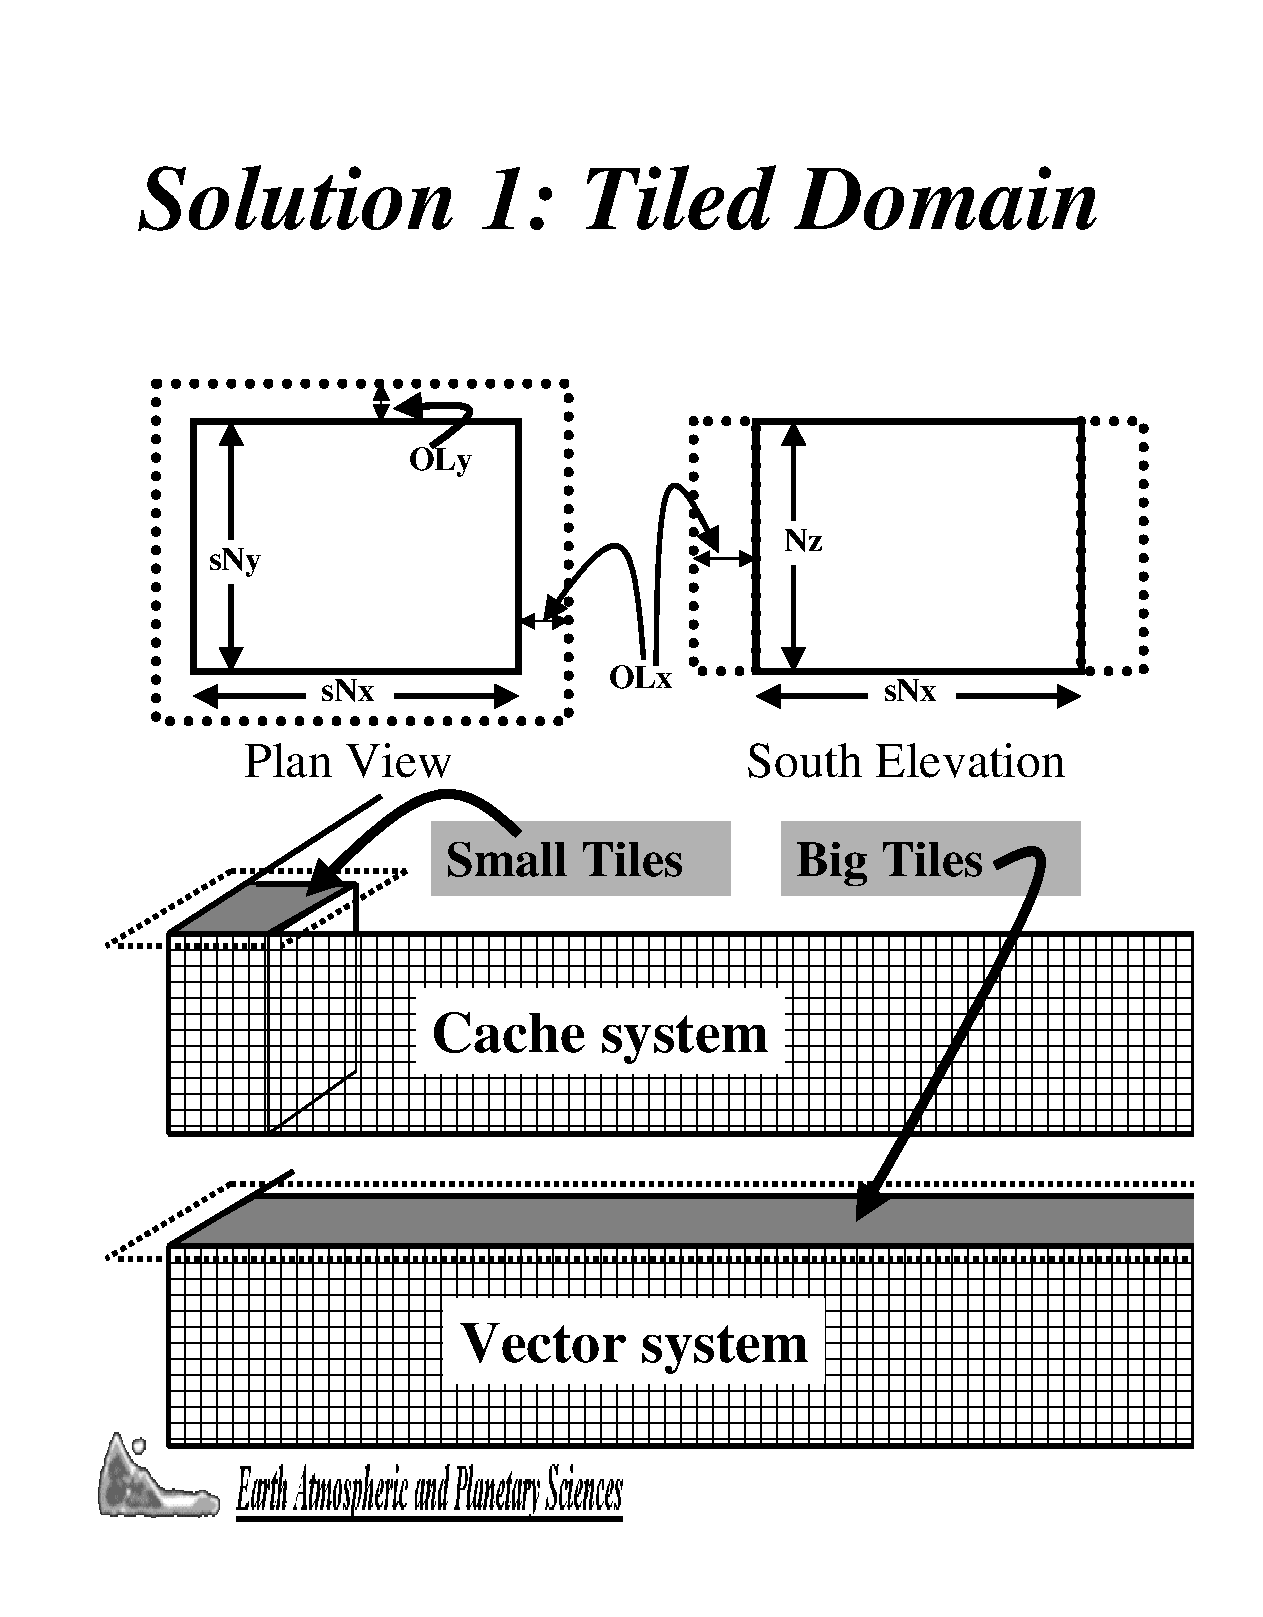
\includegraphics{part4/tiling_detail.eps}
 }
\end{center}
\caption{The tiling strategy that the WRAPPER supports allows tiles
to be shaped to suit the underlying system memory architecture.
Compact tiles that lead to greater memory reuse can be used on cache
based systems (upper half of figure) with deep memory hierarchies, long tiles 
with large inner loops can be used to exploit vector systems having
highly pipelined memory systems.
} \label{fig:tiling-strategy}
\end{figure}

\newpage
\subsection{Summary}
Following the discussion above, the machine model that the WRAPPER
presents to an application has the following characteristics

\begin{itemize}
\item The machine consists of one or more logical processors.
\item Each processor operates on tiles that it owns.
\item A processor may own more than one tile.
\item Processors may compute concurrently.
\item Exchange of information between tiles is handled by the
  machine (WRAPPER) not by the application.
\end{itemize}
Behind the scenes this allows the WRAPPER to adapt the machine model
functions to exploit hardware on which
\begin{itemize}
\item Processors may be able to communicate very efficiently with each
  other using shared memory.
\item An alternative communication mechanism based on a relatively
  simple inter-process communication API may be required.
\item Shared memory may not necessarily obey sequential consistency,
  however some mechanism will exist for enforcing memory consistency.
\item Memory consistency that is enforced at the hardware level
  may be expensive. Unnecessary triggering of consistency protocols
  should be avoided.
\item Memory access patterns may need to either repetitive or highly
  pipelined for optimum hardware performance.
\end{itemize}

This generic model captures the essential hardware ingredients
of almost all successful scientific computer systems designed in the
last 50 years.

\section{Using the WRAPPER}
\begin{rawhtml}
<!-- CMIREDIR:using_the_wrapper: -->
\end{rawhtml}

In order to support maximum portability the WRAPPER is implemented
primarily in sequential Fortran 77. At a practical level the key steps
provided by the WRAPPER are
\begin{enumerate}
\item specifying how a domain will be decomposed
\item starting a code in either sequential or parallel modes of operations
\item controlling communication between tiles and between concurrently
  computing CPUs.
\end{enumerate} 
This section describes the details of each of these operations.
Section \ref{sect:specifying_a_decomposition} explains how the way in
which a domain is decomposed (or composed) is expressed. Section
\ref{sect:starting_a_code} describes practical details of running
codes in various different parallel modes on contemporary computer
systems.  Section \ref{sect:controlling_communication} explains the
internal information that the WRAPPER uses to control how information
is communicated between tiles.

\subsection{Specifying a domain decomposition}
\label{sect:specifying_a_decomposition}

At its heart much of the WRAPPER works only in terms of a collection of tiles
which are interconnected to each other. This is also true of application
code operating within the WRAPPER. Application code is written as a series
of compute operations, each of which operates on a single tile. If
application code needs to perform operations involving data
associated with another tile, it uses a WRAPPER function to obtain
that data.
The specification of how a global domain is constructed from tiles or alternatively
how a global domain is decomposed into tiles is made in the file {\em SIZE.h}.
This file defines the following parameters \\

\fbox{ 
\begin{minipage}{4.75in}
Parameters: {\em sNx, sNy, OLx, OLy, nSx, nSy, nPx, nPy} \\
File: {\em model/inc/SIZE.h}
\end{minipage}
} \\

Together these parameters define a tiling decomposition of the style shown in 
figure \ref{fig:labelled_tile}. The parameters {\em sNx} and {\em sNy} define
the size of an individual tile. The parameters {\em OLx} and {\em OLy} define the
maximum size of the overlap extent. This must be set to the maximum width
of the computation stencil that the numerical code finite-difference operations
require between overlap region updates. The maximum overlap required
by any of the operations in the MITgcm code distributed with this release is three grid
points. This is set by the requirements of the $\nabla^4$ dissipation and 
diffusion operator. Code modifications and enhancements that involve adding wide 
finite-difference stencils may require increasing {\em OLx} and {\em OLy}.
Setting {\em OLx} and {\em OLy} to a too large value will decrease code
performance (because redundant computations will be performed), however it will
not cause any other problems.

\begin{figure}
\begin{center}
 \resizebox{5in}{!}{
  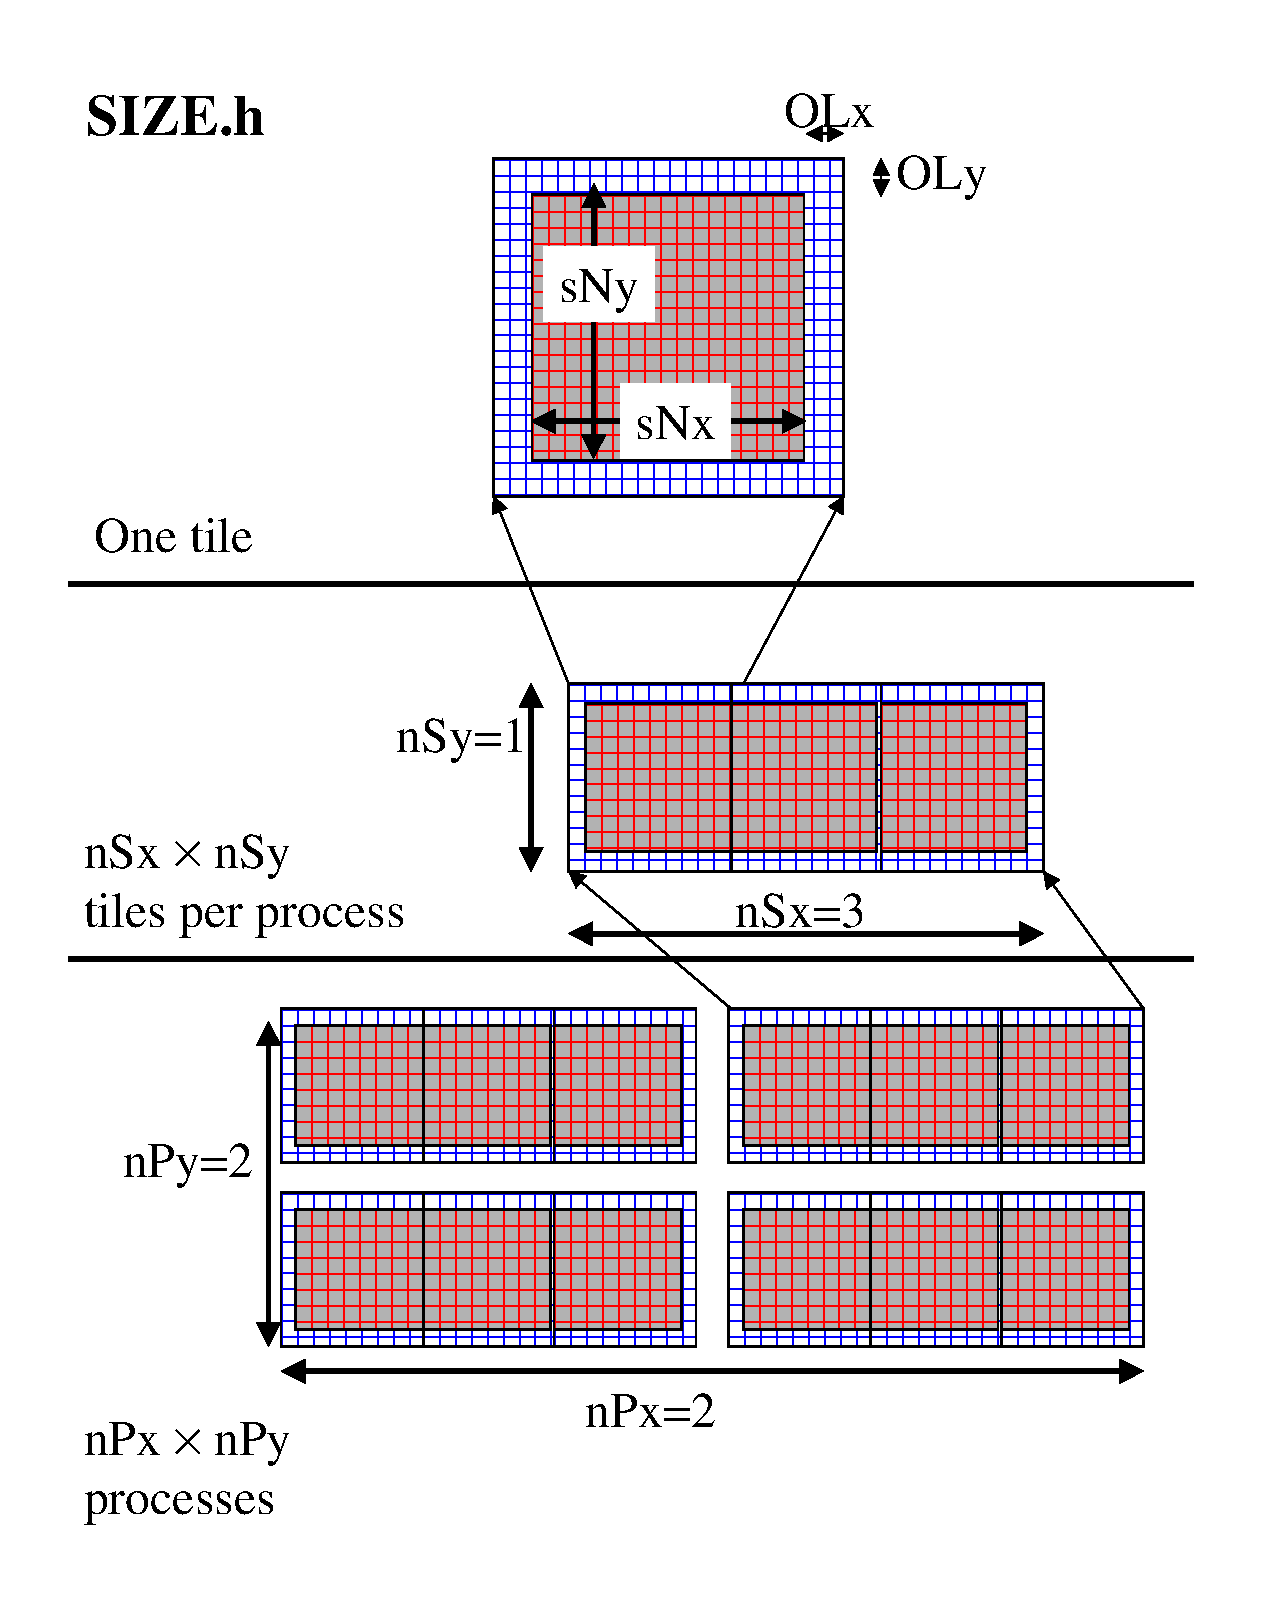
\includegraphics{part4/size_h.eps}
 }
\end{center}
\caption{ The three level domain decomposition hierarchy employed by the
WRAPPER. A domain is composed of tiles. Multiple tiles can be allocated
to a single process. Multiple processes can exist, each with multiple tiles.
Tiles within a process can be spread over multiple compute threads.
} \label{fig:labelled_tile}
\end{figure}

 The parameters {\em nSx} and {\em nSy} specify the number of tiles that will
be created within a single process. Each of these tiles will have internal
dimensions of {\em sNx} and {\em sNy}. If, when the code is executed, these tiles are 
allocated to different threads of a process that are then bound to
different physical processors ( see the multi-threaded
execution discussion in section \ref{sect:starting_the_code} ) then
computation will be performed concurrently on each tile. However, it is also
possible to run the same decomposition within a process running a single thread on
a single processor. In this case the tiles will be computed over sequentially.
If the decomposition is run in a single process running multiple threads
but attached to a single physical processor, then, in general, the computation
for different tiles will be interleaved by system level software.
This too is a valid mode of operation.

 The parameters {\em sNx, sNy, OLx, OLy, nSx} and{\em nSy} are used extensively by
numerical code. The settings of {\em sNx, sNy, OLx} and {\em OLy}
are used to form the loop ranges for many numerical calculations and
to provide dimensions for arrays holding numerical state.
The {\em nSx} and{\em nSy} are used in conjunction with the thread number
parameter {\em myThid}. Much of the numerical code operating within the
WRAPPER takes the form 
\begin{verbatim}
      DO bj=myByLo(myThid),myByHi(myThid)
       DO bi=myBxLo(myThid),myBxHi(myThid)
          :
          a block of computations ranging 
          over 1,sNx +/- OLx and 1,sNy +/- OLy grid points
          :
       ENDDO
      ENDDO

      communication code to sum a number or maybe update
      tile overlap regions

      DO bj=myByLo(myThid),myByHi(myThid)
       DO bi=myBxLo(myThid),myBxHi(myThid)
          :
          another block of computations ranging 
          over 1,sNx +/- OLx and 1,sNy +/- OLy grid points
          :
       ENDDO
      ENDDO
\end{verbatim}
The variables {\em myBxLo(myThid), myBxHi(myThid), myByLo(myThid)} and {\em
myByHi(myThid)} set the bounds of the loops in {\em bi} and {\em bj} in this 
schematic. These variables specify the subset of the tiles in
the range 1,{\em nSx} and 1,{\em nSy} that the logical processor bound to
thread number {\em myThid} owns. The thread number variable {\em myThid} 
ranges from 1 to the total number of threads requested at execution time.
For each value of {\em myThid} the loop scheme above will step sequentially
through the tiles owned by that thread. However, different threads will
have different ranges of tiles assigned to them, so that separate threads can
compute iterations of the {\em bi}, {\em bj} loop concurrently.
Within a {\em bi}, {\em bj} loop
computation is performed concurrently over as many processes and threads
as there are physical processors available to compute.

An exception to the the use of {\em bi} and {\em bj} in loops arises in the
exchange routines used when the exch2 package is used with the cubed 
sphere.  In this case {\em bj} is generally set to 1 and the loop runs from 
1,{\em bi}.  Within the loop {\em bi} is used to retrieve the tile number,
which is then used to reference exchange parameters.

The amount of computation that can be embedded
a single loop over {\em bi} and {\em bj} varies for different parts of the
MITgcm algorithm. Figure \ref{fig:bibj_extract} shows a code extract
from the two-dimensional implicit elliptic solver. This portion of the
code computes the l2Norm of a vector whose elements are held in
the array {\em cg2d\_r} writing the final result to scalar variable
{\em err}. In this case, because the l2norm requires a global reduction,
the {\em bi},{\em bj} loop only contains one statement. This computation
phase is then followed by a communication phase in which all threads and
processes must participate. However,
in other areas of the MITgcm code entries subsections of code are within
a single {\em bi},{\em bj} loop. For example the evaluation of all
the momentum equation prognostic terms ( see {\em S/R DYNAMICS()})
is within a single {\em bi},{\em bj} loop.

\begin{figure}
\begin{verbatim}
      REAL*8  cg2d_r(1-OLx:sNx+OLx,1-OLy:sNy+OLy,nSx,nSy)
      REAL*8  err
          :
          :
        other computations
          :
          :
      err = 0.
      DO bj=myByLo(myThid),myByHi(myThid)
       DO bi=myBxLo(myThid),myBxHi(myThid)
        DO J=1,sNy
         DO I=1,sNx
           err            = err            +
     &     cg2d_r(I,J,bi,bj)*cg2d_r(I,J,bi,bj)
         ENDDO
        ENDDO
       ENDDO
      ENDDO

      CALL GLOBAL_SUM_R8( err   , myThid )
      err = SQRT(err)

\end{verbatim}
\caption{Example of numerical code for calculating
the l2-norm of a vector within the WRAPPER. Notice that
under the WRAPPER arrays such as {\em cg2d\_r} have two extra trailing
dimensions. These right most indices are tile indexes. Different
threads with a single process operate on different ranges of tile
index, as controlled by the settings of
{\em myByLo, myByHi, myBxLo} and {\em myBxHi}.
} \label{fig:bibj_extract}
\end{figure}

 The final decomposition parameters are {\em nPx} and {\em nPy}. These parameters
are used to indicate to the WRAPPER level how many processes (each with
{\em nSx}$\times${\em nSy} tiles) will be used for this simulation. 
This information is needed during initialization and during I/O phases.
However, unlike the variables {\em sNx, sNy, OLx, OLy, nSx} and {\em nSy}
the values of {\em nPx} and {\em nPy} are absent
from the core numerical and support code.

\subsubsection{Examples of {\em SIZE.h} specifications}

The following different {\em SIZE.h} parameter setting illustrate how to
interpret the values of {\em sNx, sNy, OLx, OLy, nSx, nSy, nPx}
and {\em nPy}.
\begin{enumerate}
\item
\begin{verbatim}
      PARAMETER (
     &           sNx =  90,
     &           sNy =  40,
     &           OLx =   3,
     &           OLy =   3,
     &           nSx =   1,
     &           nSy =   1,
     &           nPx =   1,
     &           nPy =   1)
\end{verbatim}
This sets up a single tile with x-dimension of ninety grid points, y-dimension of
forty grid points, and x and y overlaps of three grid points each.
\item
\begin{verbatim}
      PARAMETER (
     &           sNx =  45,
     &           sNy =  20,
     &           OLx =   3,
     &           OLy =   3,
     &           nSx =   1,
     &           nSy =   1,
     &           nPx =   2,
     &           nPy =   2)
\end{verbatim}
This sets up tiles with x-dimension of forty-five grid points, y-dimension of
twenty grid points, and x and y overlaps of three grid points each. There are
four tiles allocated to four separate processes ({\em nPx=2,nPy=2}) and
arranged so that the global domain size is again ninety grid points in x and
forty grid points in y. In general the formula for global grid size (held in
model variables {\em Nx} and {\em Ny}) is
\begin{verbatim}
                 Nx  = sNx*nSx*nPx
                 Ny  = sNy*nSy*nPy
\end{verbatim}
\item
\begin{verbatim}
      PARAMETER (
     &           sNx =  90,
     &           sNy =  10,
     &           OLx =   3,
     &           OLy =   3,
     &           nSx =   1,
     &           nSy =   2,
     &           nPx =   1,
     &           nPy =   2)
\end{verbatim}
This sets up tiles with x-dimension of ninety grid points, y-dimension of
ten grid points, and x and y overlaps of three grid points each. There are
four tiles allocated to two separate processes ({\em nPy=2}) each of which
has two separate sub-domains {\em nSy=2},
The global domain size is again ninety grid points in x and
forty grid points in y. The two sub-domains in each process will be computed 
sequentially if they are given to a single thread within a single process.
Alternatively if the code is invoked with multiple threads per process
the two domains in y may be computed concurrently.
\item
\begin{verbatim}
      PARAMETER (
     &           sNx =  32,
     &           sNy =  32,
     &           OLx =   3,
     &           OLy =   3,
     &           nSx =   6,
     &           nSy =   1,
     &           nPx =   1,
     &           nPy =   1)
\end{verbatim}
This sets up tiles with x-dimension of thirty-two grid points, y-dimension of
thirty-two grid points, and x and y overlaps of three grid points each. 
There are six tiles allocated to six separate logical processors ({\em nSx=6}).
This set of values can be used for a cube sphere calculation.
Each tile of size $32 \times 32$ represents a face of the
cube. Initializing the tile connectivity correctly ( see section
\ref{sect:cube_sphere_communication}. allows the rotations associated with
moving between the six cube faces to be embedded within the 
tile-tile communication code.
\end{enumerate}


\subsection{Starting the code}
\label{sect:starting_the_code}
When code is started under the WRAPPER, execution begins in a main routine {\em
eesupp/src/main.F} that is owned by the WRAPPER. Control is transferred 
to the application through a routine called {\em THE\_MODEL\_MAIN()}
once the WRAPPER has initialized correctly and has created the necessary variables
to support subsequent calls to communication routines
by the application code. The startup calling sequence followed by the 
WRAPPER is shown in figure \ref{fig:wrapper_startup}.

\begin{figure}
{\footnotesize
\begin{verbatim}

       MAIN  
       |
       |--EEBOOT               :: WRAPPER initialization
       |  |
       |  |-- EEBOOT_MINMAL    :: Minimal startup. Just enough to
       |  |                       allow basic I/O.
       |  |-- EEINTRO_MSG      :: Write startup greeting.
       |  |
       |  |-- EESET_PARMS      :: Set WRAPPER parameters
       |  |
       |  |-- EEWRITE_EEENV    :: Print WRAPPER parameter settings
       |  |
       |  |-- INI_PROCS        :: Associate processes with grid regions.
       |  |
       |  |-- INI_THREADING_ENVIRONMENT   :: Associate threads with grid regions.
       |       |
       |       |--INI_COMMUNICATION_PATTERNS :: Initialize between tile 
       |                                     :: communication data structures
       |
       |
       |--CHECK_THREADS    :: Validate multiple thread start up.
       |
       |--THE_MODEL_MAIN   :: Numerical code top-level driver routine


\end{verbatim}
}
\caption{Main stages of the WRAPPER startup procedure.
This process proceeds transfer of control to application code, which
occurs through the procedure {\em THE\_MODEL\_MAIN()}.
} \label{fig:wrapper_startup}
\end{figure}

\subsubsection{Multi-threaded execution}
\label{sect:multi-threaded-execution}
Prior to transferring control to the procedure {\em THE\_MODEL\_MAIN()} the
WRAPPER may cause several coarse grain threads to be initialized. The routine
{\em THE\_MODEL\_MAIN()} is called once for each thread and is passed a single
stack argument which is the thread number, stored in the
variable {\em myThid}. In addition to specifying a decomposition with
multiple tiles per process ( see section \ref{sect:specifying_a_decomposition}) 
configuring and starting a code to run using multiple threads requires the following
steps.\\

\paragraph{Compilation}
First the code must be compiled with appropriate multi-threading directives 
active in the file {\em main.F} and with appropriate compiler flags
to request multi-threading support. The header files 
{\em MAIN\_PDIRECTIVES1.h} and {\em MAIN\_PDIRECTIVES2.h}
contain directives compatible with compilers for Sun, Compaq, SGI,
Hewlett-Packard SMP systems and CRAY PVP systems. These directives can be 
activated by using compile time
directives {\em -DTARGET\_SUN}, 
{\em -DTARGET\_DEC}, {\em -DTARGET\_SGI}, {\em -DTARGET\_HP}
or {\em -DTARGET\_CRAY\_VECTOR} respectively. Compiler options
for invoking multi-threaded compilation vary from system to system
and from compiler to compiler. The options will be described
in the individual compiler documentation. For the Fortran compiler 
from Sun the following options are needed to correctly compile
multi-threaded code
\begin{verbatim}
     -stackvar -explicitpar -vpara -noautopar
\end{verbatim}
These options are specific to the Sun compiler. Other compilers
will use different syntax that will be described in their
documentation. The effect of these options is as follows
\begin{enumerate}
\item {\bf -stackvar} Causes all local variables to be allocated in stack 
storage. This is necessary for local variables to ensure that they are private 
to their thread. Note, when using this option it may be necessary to override 
the default limit on stack-size that the operating system assigns to a process. 
This can normally be done by changing the settings of the command shells
{\em stack-size} limit variable. However, on some systems changing this limit
will require privileged administrator access to modify system parameters.

\item {\bf -explicitpar} Requests that multiple threads be spawned
in response to explicit directives in the application code. These
directives are inserted with syntax appropriate to the particular target
platform when, for example, the {\em -DTARGET\_SUN} flag is selected.

\item {\bf -vpara} This causes the compiler to describe the multi-threaded
configuration it is creating. This is not required
but it can be useful when trouble shooting.

\item {\bf -noautopar} This inhibits any automatic multi-threaded 
parallelization the compiler may otherwise generate.

\end{enumerate}


An example of valid settings for the {\em eedata} file for a
domain with two subdomains in y and running with two threads is shown 
below
\begin{verbatim}
 nTx=1,nTy=2
\end{verbatim}
This set of values will cause computations to stay within a single
thread when moving across the {\em nSx} sub-domains. In the y-direction,
however, sub-domains will be split equally between two threads.

\paragraph{Multi-threading files and parameters} The following
files and variables are used in setting up multi-threaded execution.\\

\fbox{ 
\begin{minipage}{4.75in}
File: {\em eesupp/inc/MAIN\_PDIRECTIVES1.h}\\
File: {\em eesupp/inc/MAIN\_PDIRECTIVES2.h}\\
File: {\em model/src/THE\_MODEL\_MAIN.F}\\
File: {\em eesupp/src/MAIN.F}\\
File: {\em tools/genmake2}\\
File: {\em eedata}\\
CPP:  {\em TARGET\_SUN}\\
CPP:  {\em TARGET\_DEC}\\
CPP:  {\em TARGET\_HP }\\
CPP:  {\em TARGET\_SGI}\\
CPP:  {\em TARGET\_CRAY\_VECTOR}\\
Parameter:  {\em nTx}\\
Parameter:  {\em nTy}
\end{minipage}
} \\

\subsubsection{Multi-process execution}
\label{sect:multi-process-execution}

Despite its appealing programming model, multi-threaded execution
remains less common than multi-process execution. One major reason for
this is that many system libraries are still not ``thread-safe''. This
means that, for example, on some systems it is not safe to call system
routines to perform I/O when running in multi-threaded mode (except,
perhaps, in a limited set of circumstances).  Another reason is that
support for multi-threaded programming models varies between systems.

Multi-process execution is more ubiquitous.  In order to run code in a
multi-process configuration a decomposition specification (see section
\ref{sect:specifying_a_decomposition}) is given (in which the at least
one of the parameters {\em nPx} or {\em nPy} will be greater than one)
and then, as for multi-threaded operation, appropriate compile time
and run time steps must be taken.

\paragraph{Compilation} Multi-process execution under the WRAPPER
assumes that the portable, MPI libraries are available for controlling
the start-up of multiple processes. The MPI libraries are not
required, although they are usually used, for performance critical
communication. However, in order to simplify the task of controlling
and coordinating the start up of a large number (hundreds and possibly
even thousands) of copies of the same program, MPI is used. The calls
to the MPI multi-process startup routines must be activated at compile
time.  Currently MPI libraries are invoked by specifying the
appropriate options file with the {\tt-of} flag when running the {\em
  genmake2} script, which generates the Makefile for compiling and
linking MITgcm.  (Previously this was done by setting the {\em
  ALLOW\_USE\_MPI} and {\em ALWAYS\_USE\_MPI} flags in the {\em
  CPP\_EEOPTIONS.h} file.)  More detailed information about the use of
{\em genmake2} for specifying
local compiler flags is located in section \ref{sect:genmake}.\\


\fbox{ 
\begin{minipage}{4.75in}
Directory: {\em tools/build\_options}\\
File: {\em tools/genmake2}
\end{minipage}
} \\
\paragraph{\bf Execution} The mechanics of starting a program in
multi-process mode under MPI is not standardized. Documentation
associated with the distribution of MPI installed on a system will
describe how to start a program using that distribution.  For the
open-source MPICH system, the MITgcm program can be started using a
command such as
\begin{verbatim}
mpirun -np 64 -machinefile mf ./mitgcmuv
\end{verbatim}
In this example the text {\em -np 64} specifies the number of
processes that will be created. The numeric value {\em 64} must be
equal to the product of the processor grid settings of {\em nPx} and
{\em nPy} in the file {\em SIZE.h}. The parameter {\em mf} specifies
that a text file called ``mf'' will be read to get a list of processor
names on which the sixty-four processes will execute. The syntax of
this file is specified by the MPI distribution.
\\

\fbox{ 
\begin{minipage}{4.75in}
File: {\em SIZE.h}\\
Parameter: {\em nPx}\\
Parameter: {\em nPy}
\end{minipage}
} \\


\paragraph{Environment variables}
On most systems multi-threaded execution also requires the setting of
a special environment variable. On many machines this variable is
called PARALLEL and its values should be set to the number of parallel
threads required. Generally the help or manual pages associated with
the multi-threaded compiler on a machine will explain how to set the
required environment variables.

\paragraph{Runtime input parameters}
Finally the file {\em eedata} needs to be configured to indicate the
number of threads to be used in the x and y directions.  The variables
{\em nTx} and {\em nTy} in this file are used to specify the
information required. The product of {\em nTx} and {\em nTy} must be
equal to the number of threads spawned i.e.  the setting of the
environment variable PARALLEL.  The value of {\em nTx} must subdivide
the number of sub-domains in x ({\em nSx}) exactly. The value of {\em
  nTy} must subdivide the number of sub-domains in y ({\em nSy})
exactly.  The multiprocess startup of the MITgcm executable {\em
  mitgcmuv} is controlled by the routines {\em EEBOOT\_MINIMAL()} and
{\em INI\_PROCS()}. The first routine performs basic steps required to
make sure each process is started and has a textual output stream
associated with it. By default two output files are opened for each
process with names {\bf STDOUT.NNNN} and {\bf STDERR.NNNN}.  The {\bf
  NNNNN} part of the name is filled in with the process number so that
process number 0 will create output files {\bf STDOUT.0000} and {\bf
  STDERR.0000}, process number 1 will create output files {\bf
  STDOUT.0001} and {\bf STDERR.0001}, etc. These files are used for
reporting status and configuration information and for reporting error
conditions on a process by process basis.  The {\em EEBOOT\_MINIMAL()}
procedure also sets the variables {\em myProcId} and {\em
  MPI\_COMM\_MODEL}.  These variables are related to processor
identification are are used later in the routine {\em INI\_PROCS()} to
allocate tiles to processes.

Allocation of processes to tiles is controlled by the routine {\em
  INI\_PROCS()}. For each process this routine sets the variables {\em
  myXGlobalLo} and {\em myYGlobalLo}.  These variables specify, in
index space, the coordinates of the southernmost and westernmost
corner of the southernmost and westernmost tile owned by this process.
The variables {\em pidW}, {\em pidE}, {\em pidS} and {\em pidN} are
also set in this routine. These are used to identify processes holding
tiles to the west, east, south and north of a given process. These
values are stored in global storage in the header file {\em
  EESUPPORT.h} for use by communication routines.  The above does not
hold when the exch2 package is used.  The exch2 sets its own
parameters to specify the global indices of tiles and their
relationships to each other.  See the documentation on the exch2
package (\ref{sec:exch2}) for details.
\\

\fbox{ 
\begin{minipage}{4.75in}
File: {\em eesupp/src/eeboot\_minimal.F}\\
File: {\em eesupp/src/ini\_procs.F} \\
File: {\em eesupp/inc/EESUPPORT.h} \\
Parameter: {\em myProcId} \\
Parameter: {\em MPI\_COMM\_MODEL} \\
Parameter: {\em myXGlobalLo} \\
Parameter: {\em myYGlobalLo} \\
Parameter: {\em pidW       } \\
Parameter: {\em pidE       } \\
Parameter: {\em pidS       } \\
Parameter: {\em pidN       }
\end{minipage}
} \\


\subsection{Controlling communication}
The WRAPPER maintains internal information that is used for communication
operations and that can be customized for different platforms. This section 
describes the information that is held and used.

\begin{enumerate}
\item {\bf Tile-tile connectivity information}
  For each tile the WRAPPER sets a flag that sets the tile number to
  the north, south, east and west of that tile. This number is unique
  over all tiles in a configuration. Except when using the cubed
  sphere and the exch2 package, the number is held in the variables
  {\em tileNo} ( this holds the tiles own number), {\em tileNoN}, {\em
    tileNoS}, {\em tileNoE} and {\em tileNoW}. A parameter is also
  stored with each tile that specifies the type of communication that
  is used between tiles.  This information is held in the variables
  {\em tileCommModeN}, {\em tileCommModeS}, {\em tileCommModeE} and
  {\em tileCommModeW}.  This latter set of variables can take one of
  the following values {\em COMM\_NONE}, {\em COMM\_MSG}, {\em
    COMM\_PUT} and {\em COMM\_GET}.  A value of {\em COMM\_NONE} is
  used to indicate that a tile has no neighbor to communicate with on
  a particular face. A value of {\em COMM\_MSG} is used to indicate
  that some form of distributed memory communication is required to
  communicate between these tile faces (see section
  \ref{sect:distributed_memory_communication}).  A value of {\em
    COMM\_PUT} or {\em COMM\_GET} is used to indicate forms of shared
  memory communication (see section
  \ref{sect:shared_memory_communication}). The {\em COMM\_PUT} value
  indicates that a CPU should communicate by writing to data
  structures owned by another CPU. A {\em COMM\_GET} value indicates
  that a CPU should communicate by reading from data structures owned
  by another CPU. These flags affect the behavior of the WRAPPER
  exchange primitive (see figure \ref{fig:communication_primitives}).
  The routine {\em ini\_communication\_patterns()} is responsible for
  setting the communication mode values for each tile.

  When using the cubed sphere configuration with the exch2 package,
  the relationships between tiles and their communication methods are
  set by the exch2 package and stored in different variables.  See the
  exch2 package documentation (\ref{sec:exch2} for details.

\fbox{ 
\begin{minipage}{4.75in}
File: {\em eesupp/src/ini\_communication\_patterns.F}\\
File: {\em eesupp/inc/EESUPPORT.h} \\
Parameter: {\em tileNo} \\
Parameter: {\em tileNoE} \\
Parameter: {\em tileNoW} \\
Parameter: {\em tileNoN} \\
Parameter: {\em tileNoS} \\
Parameter: {\em tileCommModeE} \\
Parameter: {\em tileCommModeW} \\
Parameter: {\em tileCommModeN} \\
Parameter: {\em tileCommModeS} \\
\end{minipage}
} \\

\item {\bf MP directives}
  The WRAPPER transfers control to numerical application code through
  the routine {\em THE\_MODEL\_MAIN}. This routine is called in a way
  that allows for it to be invoked by several threads. Support for
  this is based on either multi-processing (MP) compiler directives or
  specific calls to multi-threading libraries (\textit{eg.} POSIX
  threads).  Most commercially available Fortran compilers support the
  generation of code to spawn multiple threads through some form of
  compiler directives.  Compiler directives are generally more
  convenient than writing code to explicitly spawning threads.  And,
  on some systems, compiler directives may be the only method
  available.  The WRAPPER is distributed with template MP directives
  for a number of systems.

  These directives are inserted into the code just before and after
  the transfer of control to numerical algorithm code through the
  routine {\em THE\_MODEL\_MAIN}. Figure \ref{fig:mp_directives} shows
  an example of the code that performs this process for a Silicon
  Graphics system.  This code is extracted from the files {\em main.F}
  and {\em MAIN\_PDIRECTIVES1.h}. The variable {\em nThreads}
  specifies how many instances of the routine {\em THE\_MODEL\_MAIN}
  will be created. The value of {\em nThreads} is set in the routine
  {\em INI\_THREADING\_ENVIRONMENT}. The value is set equal to the the
  product of the parameters {\em nTx} and {\em nTy} that are read from
  the file {\em eedata}. If the value of {\em nThreads} is
  inconsistent with the number of threads requested from the operating
  system (for example by using an environment variable as described in
  section \ref{sect:multi_threaded_execution}) then usually an error
  will be reported by the routine {\em CHECK\_THREADS}.

\fbox{ 
\begin{minipage}{4.75in}
File: {\em eesupp/src/ini\_threading\_environment.F}\\
File: {\em eesupp/src/check\_threads.F} \\
File: {\em eesupp/src/main.F} \\
File: {\em eesupp/inc/MAIN\_PDIRECTIVES1.h} \\
File: {\em eedata           } \\
Parameter: {\em nThreads} \\
Parameter: {\em nTx} \\
Parameter: {\em nTy} \\
\end{minipage}
}

\item {\bf memsync flags}
  As discussed in section \ref{sect:memory_consistency}, a low-level
  system function may be need to force memory consistency on some
  shared memory systems.  The routine {\em MEMSYNC()} is used for this
  purpose. This routine should not need modifying and the information
  below is only provided for completeness. A logical parameter {\em
    exchNeedsMemSync} set in the routine {\em
    INI\_COMMUNICATION\_PATTERNS()} controls whether the {\em
    MEMSYNC()} primitive is called. In general this routine is only
  used for multi-threaded execution.  The code that goes into the {\em
    MEMSYNC()} routine is specific to the compiler and processor used.
  In some cases, it must be written using a short code snippet of
  assembly language.  For an Ultra Sparc system the following code
  snippet is used
\begin{verbatim}
asm("membar #LoadStore|#StoreStore");
\end{verbatim}
for an Alpha based system the equivalent code reads
\begin{verbatim}
asm("mb");
\end{verbatim}
while on an x86 system the following code is required
\begin{verbatim}
asm("lock; addl $0,0(%%esp)": : :"memory")
\end{verbatim}

\item {\bf Cache line size}
  As discussed in section \ref{sect:cache_effects_and_false_sharing},
  milti-threaded codes explicitly avoid penalties associated with
  excessive coherence traffic on an SMP system. To do this the shared
  memory data structures used by the {\em GLOBAL\_SUM}, {\em
    GLOBAL\_MAX} and {\em BARRIER} routines are padded. The variables
  that control the padding are set in the header file {\em
    EEPARAMS.h}. These variables are called {\em cacheLineSize}, {\em
    lShare1}, {\em lShare4} and {\em lShare8}. The default values
  should not normally need changing.

\item {\bf \_BARRIER}
  This is a CPP macro that is expanded to a call to a routine which
  synchronizes all the logical processors running under the WRAPPER.
  Using a macro here preserves flexibility to insert a specialized
  call in-line into application code. By default this resolves to
  calling the procedure {\em BARRIER()}. The default setting for the
  \_BARRIER macro is given in the file {\em CPP\_EEMACROS.h}.

\item {\bf \_GSUM}
  This is a CPP macro that is expanded to a call to a routine which
  sums up a floating point number over all the logical processors
  running under the WRAPPER. Using a macro here provides extra
  flexibility to insert a specialized call in-line into application
  code. By default this resolves to calling the procedure {\em
    GLOBAL\_SUM\_R8()} ( for 64-bit floating point operands) or {\em
    GLOBAL\_SUM\_R4()} (for 32-bit floating point operands). The
  default setting for the \_GSUM macro is given in the file {\em
    CPP\_EEMACROS.h}.  The \_GSUM macro is a performance critical
  operation, especially for large processor count, small tile size
  configurations.  The custom communication example discussed in
  section \ref{sect:jam_example} shows how the macro is used to invoke
  a custom global sum routine for a specific set of hardware.

\item {\bf \_EXCH}
  The \_EXCH CPP macro is used to update tile overlap regions.  It is
  qualified by a suffix indicating whether overlap updates are for
  two-dimensional ( \_EXCH\_XY ) or three dimensional ( \_EXCH\_XYZ )
  physical fields and whether fields are 32-bit floating point (
  \_EXCH\_XY\_R4, \_EXCH\_XYZ\_R4 ) or 64-bit floating point (
  \_EXCH\_XY\_R8, \_EXCH\_XYZ\_R8 ). The macro mappings are defined in
  the header file {\em CPP\_EEMACROS.h}. As with \_GSUM, the \_EXCH
  operation plays a crucial role in scaling to small tile, large
  logical and physical processor count configurations.  The example in
  section \ref{sect:jam_example} discusses defining an optimized and
  specialized form on the \_EXCH operation.

  The \_EXCH operation is also central to supporting grids such as the
  cube-sphere grid. In this class of grid a rotation may be required
  between tiles. Aligning the coordinate requiring rotation with the
  tile decomposition, allows the coordinate transformation to be
  embedded within a custom form of the \_EXCH primitive.  In these
  cases \_EXCH is mapped to exch2 routines, as detailed in the exch2
  package documentation \ref{sec:exch2}.

\item {\bf Reverse Mode}
  The communication primitives \_EXCH and \_GSUM both employ
  hand-written adjoint forms (or reverse mode) forms.  These reverse
  mode forms can be found in the source code directory {\em
    pkg/autodiff}.  For the global sum primitive the reverse mode form
  calls are to {\em GLOBAL\_ADSUM\_R4} and {\em GLOBAL\_ADSUM\_R8}.
  The reverse mode form of the exchange primitives are found in
  routines prefixed {\em ADEXCH}. The exchange routines make calls to
  the same low-level communication primitives as the forward mode
  operations. However, the routine argument {\em simulationMode} is
  set to the value {\em REVERSE\_SIMULATION}. This signifies to the
  low-level routines that the adjoint forms of the appropriate
  communication operation should be performed.

\item {\bf MAX\_NO\_THREADS}
  The variable {\em MAX\_NO\_THREADS} is used to indicate the maximum
  number of OS threads that a code will use. This value defaults to
  thirty-two and is set in the file {\em EEPARAMS.h}.  For single
  threaded execution it can be reduced to one if required.  The value
  is largely private to the WRAPPER and application code will not
  normally reference the value, except in the following scenario.

  For certain physical parametrization schemes it is necessary to have
  a substantial number of work arrays. Where these arrays are
  allocated in heap storage (for example COMMON blocks) multi-threaded
  execution will require multiple instances of the COMMON block data.
  This can be achieved using a Fortran 90 module construct.  However,
  if this mechanism is unavailable then the work arrays can be extended
  with dimensions using the tile dimensioning scheme of {\em nSx} and
  {\em nSy} (as described in section
  \ref{sect:specifying_a_decomposition}). However, if the
  configuration being specified involves many more tiles than OS
  threads then it can save memory resources to reduce the variable
  {\em MAX\_NO\_THREADS} to be equal to the actual number of threads
  that will be used and to declare the physical parameterization work
  arrays with a single {\em MAX\_NO\_THREADS} extra dimension.  An
  example of this is given in the verification experiment {\em
    aim.5l\_cs}. Here the default setting of {\em MAX\_NO\_THREADS} is
  altered to
\begin{verbatim}
      INTEGER MAX_NO_THREADS
      PARAMETER ( MAX_NO_THREADS =    6 )
\end{verbatim}
  and several work arrays for storing intermediate calculations are
  created with declarations of the form.
\begin{verbatim}
      common /FORCIN/ sst1(ngp,MAX_NO_THREADS)
\end{verbatim}
  This declaration scheme is not used widely, because most global data
  is used for permanent not temporary storage of state information.
  In the case of permanent state information this approach cannot be
  used because there has to be enough storage allocated for all tiles.
  However, the technique can sometimes be a useful scheme for reducing
  memory requirements in complex physical parameterizations.
\end{enumerate}

\begin{figure}
\begin{verbatim}
C--
C--  Parallel directives for MIPS Pro Fortran compiler
C--
C      Parallel compiler directives for SGI with IRIX
C$PAR  PARALLEL DO
C$PAR&  CHUNK=1,MP_SCHEDTYPE=INTERLEAVE,
C$PAR&  SHARE(nThreads),LOCAL(myThid,I)
C
      DO I=1,nThreads
        myThid = I

C--     Invoke nThreads instances of the numerical model
        CALL THE_MODEL_MAIN(myThid)

      ENDDO
\end{verbatim}
  \caption{Prior to transferring control to the procedure {\em
      THE\_MODEL\_MAIN()} the WRAPPER may use MP directives to spawn
    multiple threads.  } \label{fig:mp_directives}
\end{figure}


\subsubsection{Specializing the Communication Code}

The isolation of performance critical communication primitives and the
sub-division of the simulation domain into tiles is a powerful tool.
Here we show how it can be used to improve application performance and
how it can be used to adapt to new griding approaches.

\subsubsection{JAM example}
\label{sect:jam_example}
On some platforms a big performance boost can be obtained by binding
the communication routines {\em \_EXCH} and {\em \_GSUM} to
specialized native libraries (for example, the shmem library on CRAY
T3E systems). The {\em LETS\_MAKE\_JAM} CPP flag is used as an
illustration of a specialized communication configuration that
substitutes for standard, portable forms of {\em \_EXCH} and {\em
  \_GSUM}. It affects three source files {\em eeboot.F}, {\em
  CPP\_EEMACROS.h} and {\em cg2d.F}. When the flag is defined is has
the following effects.
\begin{itemize}
\item An extra phase is included at boot time to initialize the custom
  communications library ( see {\em ini\_jam.F}).
\item The {\em \_GSUM} and {\em \_EXCH} macro definitions are replaced
  with calls to custom routines (see {\em gsum\_jam.F} and {\em
    exch\_jam.F})
\item a highly specialized form of the exchange operator (optimized
  for overlap regions of width one) is substituted into the elliptic
  solver routine {\em cg2d.F}.
\end{itemize}
Developing specialized code for other libraries follows a similar
pattern.

\subsubsection{Cube sphere communication}
\label{sect:cube_sphere_communication}
Actual {\em \_EXCH} routine code is generated automatically from a
series of template files, for example {\em exch\_rx.template}.  This
is done to allow a large number of variations on the exchange process
to be maintained. One set of variations supports the cube sphere grid.
Support for a cube sphere grid in MITgcm is based on having each face
of the cube as a separate tile or tiles.  The exchange routines are
then able to absorb much of the detailed rotation and reorientation
required when moving around the cube grid. The set of {\em \_EXCH}
routines that contain the word cube in their name perform these
transformations.  They are invoked when the run-time logical parameter
{\em useCubedSphereExchange} is set true. To facilitate the
transformations on a staggered C-grid, exchange operations are defined
separately for both vector and scalar quantities and for grid-centered
and for grid-face and grid-corner quantities.  Three sets of exchange
routines are defined. Routines with names of the form {\em exch\_rx}
are used to exchange cell centered scalar quantities. Routines with
names of the form {\em exch\_uv\_rx} are used to exchange vector
quantities located at the C-grid velocity points. The vector
quantities exchanged by the {\em exch\_uv\_rx} routines can either be
signed (for example velocity components) or un-signed (for example
grid-cell separations).  Routines with names of the form {\em
  exch\_z\_rx} are used to exchange quantities at the C-grid vorticity
point locations.




\section{MITgcm execution under WRAPPER}
\begin{rawhtml}
<!-- CMIREDIR:mitgcm_wrapper: -->
\end{rawhtml}

Fitting together the WRAPPER elements, package elements and
MITgcm core equation elements of the source code produces calling
sequence shown in section \ref{sect:calling_sequence}

\subsection{Annotated call tree for MITgcm and WRAPPER}
\label{sect:calling_sequence}

WRAPPER layer.

{\footnotesize
\begin{verbatim}

       MAIN  
       |
       |--EEBOOT               :: WRAPPER initialization
       |  |
       |  |-- EEBOOT_MINMAL    :: Minimal startup. Just enough to
       |  |                       allow basic I/O.
       |  |-- EEINTRO_MSG      :: Write startup greeting.
       |  |
       |  |-- EESET_PARMS      :: Set WRAPPER parameters
       |  |
       |  |-- EEWRITE_EEENV    :: Print WRAPPER parameter settings
       |  |
       |  |-- INI_PROCS        :: Associate processes with grid regions.
       |  |
       |  |-- INI_THREADING_ENVIRONMENT   :: Associate threads with grid regions.
       |       |
       |       |--INI_COMMUNICATION_PATTERNS :: Initialize between tile 
       |                                     :: communication data structures
       |
       |
       |--CHECK_THREADS    :: Validate multiple thread start up.
       |
       |--THE_MODEL_MAIN   :: Numerical code top-level driver routine

\end{verbatim}
}

Core equations plus packages.

{\footnotesize
\begin{verbatim}
C
C Invocation from WRAPPER level...
C  :
C  :
C  |
C  |-THE_MODEL_MAIN :: Primary driver for the MITgcm algorithm
C    |              :: Called from WRAPPER level numerical
C    |              :: code invocation routine. On entry
C    |              :: to THE_MODEL_MAIN separate thread and
C    |              :: separate processes will have been established.
C    |              :: Each thread and process will have a unique ID
C    |              :: but as yet it will not be associated with a
C    |              :: specific region in decomposed discrete space.
C    |
C    |-INITIALISE_FIXED :: Set fixed model arrays such as topography, 
C    | |                :: grid, solver matrices etc..
C    | |              
C    | |-INI_PARMS :: Routine to set kernel model parameters.
C    | |           :: By default kernel parameters are read from file 
C    | |           :: "data" in directory in which code executes.
C    | |
C    | |-MON_INIT :: Initializes monitor package ( see pkg/monitor )
C    | |
C    | |-INI_GRID :: Control grid array (vert. and hori.) initialization.
C    | | |        :: Grid arrays are held and described in GRID.h.
C    | | |
C    | | |-INI_VERTICAL_GRID        :: Initialize vertical grid arrays.
C    | | |
C    | | |-INI_CARTESIAN_GRID       :: Cartesian horiz. grid initialization
C    | | |                          :: (calculate grid from kernel parameters).
C    | | |
C    | | |-INI_SPHERICAL_POLAR_GRID :: Spherical polar horiz. grid 
C    | | |                          :: initialization (calculate grid from 
C    | | |                          :: kernel parameters).
C    | | |
C    | | |-INI_CURVILINEAR_GRID     :: General orthogonal, structured horiz.
C    | |                            :: grid initializations. ( input from raw
C    | |                            :: grid files, LONC.bin, DXF.bin etc... )
C    | |
C    | |-INI_DEPTHS    :: Read (from "bathyFile") or set bathymetry/orgography.
C    | |
C    | |-INI_MASKS_ETC :: Derive horizontal and vertical cell fractions and
C    | |               :: land masking for solid-fluid boundaries.
C    | |
C    | |-INI_LINEAR_PHSURF :: Set ref. surface Bo_surf
C    | |
C    | |-INI_CORI          :: Set coriolis term. zero, f-plane, beta-plane,
C    | |                   :: sphere options are coded.
C    | |
C    | |-PACAKGES_BOOT      :: Start up the optional package environment.
C    | |                    :: Runtime selection of active packages.
C    | |
C    | |-PACKAGES_READPARMS :: Call active package internal parameter load.
C    | | |
C    | | |-GMREDI_READPARMS    :: GM Package. see pkg/gmredi
C    | | |-KPP_READPARMS       :: KPP Package. see pkg/kpp
C    | | |-SHAP_FILT_READPARMS :: Shapiro filter package. see pkg/shap_filt
C    | | |-OBCS_READPARMS      :: Open bndy package. see pkg/obcs
C    | | |-AIM_READPARMS       :: Intermediate Atmos. pacakage. see pkg/aim
C    | | |-COST_READPARMS      :: Cost function package. see pkg/cost
C    | | |-CTRL_INIT           :: Control vector support package. see pkg/ctrl
C    | | |-OPTIM_READPARMS     :: Optimisation support package. see pkg/ctrl 
C    | | |-GRDCHK_READPARMS    :: Gradient check package. see pkg/grdchk
C    | | |-ECCO_READPARMS      :: ECCO Support Package. see pkg/ecco
C    | | |-PTRACERS_READPARMS  :: multiple tracer package, see pkg/ptracers
C    | | |-GCHEM_READPARMS     :: tracer interface package, see pkg/gchem
C    | |
C    | |-PACKAGES_CHECK
C    | | |
C    | | |-KPP_CHECK           :: KPP Package. pkg/kpp
C    | | |-OBCS_CHECK          :: Open bndy Pacakge. pkg/obcs
C    | | |-GMREDI_CHECK        :: GM Package. pkg/gmredi
C    | |
C    | |-PACKAGES_INIT_FIXED
C    | | |-OBCS_INIT_FIXED     :: Open bndy Package. see pkg/obcs
C    | | |-FLT_INIT            :: Floats Package. see pkg/flt
C    | | |-GCHEM_INIT_FIXED    :: tracer interface pachage, see pkg/gchem
C    | |
C    | |-ZONAL_FILT_INIT       :: FFT filter Package. see pkg/zonal_filt
C    | |
C    | |-INI_CG2D              :: 2d con. grad solver initialization.
C    | |
C    | |-INI_CG3D              :: 3d con. grad solver initialization.
C    | |
C    | |-CONFIG_SUMMARY        :: Provide synopsis of kernel setup.
C    |                         :: Includes annotated table of kernel 
C    |                         :: parameter settings.
C    |
C    |-CTRL_UNPACK :: Control vector support package. see pkg/ctrl
C    |
C    |-ADTHE_MAIN_LOOP :: Derivative evaluating form of main time stepping loop
C    !                 :: Auotmatically generated by TAMC/TAF.
C    |
C    |-CTRL_PACK   :: Control vector support package. see pkg/ctrl
C    |
C    |-GRDCHK_MAIN :: Gradient check package. see pkg/grdchk
C    |
C    |-THE_MAIN_LOOP :: Main timestepping loop routine.
C    | |
C    | |-INITIALISE_VARIA :: Set the initial conditions for time evolving 
C    | | |                :: variables
C    | | |
C    | | |-INI_LINEAR_PHISURF :: Set ref. surface Bo_surf
C    | | |
C    | | |-INI_CORI     :: Set coriolis term. zero, f-plane, beta-plane,
C    | | |              :: sphere options are coded.
C    | | |
C    | | |-INI_CG2D     :: 2d con. grad solver initialization.
C    | | |-INI_CG3D     :: 3d con. grad solver initialization.
C    | | |-INI_MIXING   :: Initialize diapycnal diffusivity.
C    | | |-INI_DYNVARS  :: Initialize to zero all DYNVARS.h arrays (dynamical
C    | | |              :: fields).
C    | | |
C    | | |-INI_FIELDS   :: Control initializing model fields to non-zero
C    | | | |-INI_VEL    :: Initialize 3D flow field.
C    | | | |-INI_THETA  :: Set model initial temperature field.
C    | | | |-INI_SALT   :: Set model initial salinity field.
C    | | | |-INI_PSURF  :: Set model initial free-surface height/pressure.
C    | | | |-INI_PRESSURE :: Compute model initial hydrostatic pressure
C    | | | |-READ_CHECKPOINT :: Read the checkpoint
C    | | |
C    | | |-THE_CORRECTION_STEP :: Step forward to next time step.
C    | | | |                   :: Here applied to move restart conditions
C    | | | |                   :: (saved in mid timestep) to correct level in 
C    | | | |                   :: time (only used for pre-c35).
C    | | | |
C    | | | |-CALC_GRAD_PHI_SURF :: Return DDx and DDy of surface pressure
C    | | | |-CORRECTION_STEP    :: Pressure correction to momentum
C    | | | |-CYCLE_TRACER       :: Move tracers forward in time.
C    | | | |-OBCS_APPLY         :: Open bndy package. see pkg/obcs
C    | | | |-SHAP_FILT_APPLY    :: Shapiro filter package. see pkg/shap_filt
C    | | | |-ZONAL_FILT_APPLY   :: FFT filter package. see pkg/zonal_filt
C    | | | |-CONVECTIVE_ADJUSTMENT :: Control static instability mixing.
C    | | | | |-FIND_RHO  :: Find adjacent densities.
C    | | | | |-CONVECT   :: Mix static instability.
C    | | | | |-TIMEAVE_CUMULATE :: Update convection statistics.
C    | | | | 
C    | | | |-CALC_EXACT_ETA        :: Change SSH to flow divergence.     
C    | | | 
C    | | |-CONVECTIVE_ADJUSTMENT_INI :: Control static instability mixing
C    | | | |                         :: Extra time history interactions.
C    | | | |                       
C    | | | |-FIND_RHO  :: Find adjacent densities.
C    | | | |-CONVECT   :: Mix static instability.
C    | | | |-TIMEAVE_CUMULATE :: Update convection statistics.
C    | | |
C    | | |-PACKAGES_INIT_VARIABLES :: Does initialization of time evolving 
C    | | | |                       :: package data.
C    | | | |
C    | | | |-GMREDI_INIT          :: GM package. ( see pkg/gmredi )
C    | | | |-KPP_INIT             :: KPP package. ( see pkg/kpp )
C    | | | |-KPP_OPEN_DIAGS    
C    | | | |-OBCS_INIT_VARIABLES  :: Open bndy. package. ( see pkg/obcs )
C    | | | |-PTRACERS_INIT        :: multi. tracer package,(see pkg/ptracers)
C    | | | |-GCHEM_INIT           :: tracer interface pkg (see pkh/gchem)
C    | | | |-AIM_INIT             :: Interm. atmos package. ( see pkg/aim )
C    | | | |-CTRL_MAP_INI         :: Control vector package.( see pkg/ctrl )
C    | | | |-COST_INIT            :: Cost function package. ( see pkg/cost )
C    | | | |-ECCO_INIT            :: ECCO support package. ( see pkg/ecco )
C    | | | |-INI_FORCING          :: Set model initial forcing fields.
C    | | |   |                    :: Either set in-line or from file as shown.
C    | | |   |-READ_FLD_XY_RS(zonalWindFile)
C    | | |   |-READ_FLD_XY_RS(meridWindFile)
C    | | |   |-READ_FLD_XY_RS(surfQFile)
C    | | |   |-READ_FLD_XY_RS(EmPmRfile)
C    | | |   |-READ_FLD_XY_RS(thetaClimFile)
C    | | |   |-READ_FLD_XY_RS(saltClimFile)
C    | | |   |-READ_FLD_XY_RS(surfQswFile)
C    | | |
C    | | |-CALC_SURF_DR   :: Calculate the new surface level thickness.
C    | | |-UPDATE_SURF_DR :: Update the surface-level thickness fraction.
C    | | |-UPDATE_CG2D    :: Update 2d conjugate grad. for Free-Surf.
C    | | |-STATE_SUMMARY    :: Summarize model prognostic variables.
C    | | |-TIMEAVE_STATVARS :: Time averaging package ( see pkg/timeave ).
C    | |
C    | |-WRITE_STATE      :: Controlling routine for IO to dump model state.
C    | | |-WRITE_REC_XYZ_RL :: Single file I/O
C    | | |-WRITE_FLD_XYZ_RL :: Multi-file I/O
C    | | 
C    | |-MONITOR          :: Monitor state ( see pkg/monitor )
C    | |-CTRL_MAP_FORCING :: Control vector support package. ( see pkg/ctrl )
C====|>| 
C====|>| ****************************
C====|>| BEGIN MAIN TIMESTEPPING LOOP
C====|>| ****************************
C====|>| 
C/\  | |-FORWARD_STEP     :: Step forward a time-step ( AT LAST !!! )
C/\  | | |
C/\  | | |-DUMMY_IN_STEPPING :: autodiff package ( pkg/autoduff ).
C/\  | | |-CALC_EXACT_ETA :: Change SSH to flow divergence.
C/\  | | |-CALC_SURF_DR   :: Calculate the new surface level thickness.
C/\  | | |-EXF_GETFORCING :: External forcing package. ( pkg/exf )
C/\  | | |-EXTERNAL_FIELDS_LOAD :: Control loading time dep. external data.
C/\  | | | |                    :: Simple interpolation between end-points 
C/\  | | | |                    :: for forcing datasets.
C/\  | | | |                  
C/\  | | | |-EXCH :: Sync forcing. in overlap regions.
C/\  | | |-SEAICE_MODEL   :: Compute sea-ice terms. ( pkg/seaice )
C/\  | | |-FREEZE         :: Limit surface temperature.
C/\  | | |-GCHEM_FIELD_LOAD :: load tracer forcing fields (pkg/gchem)
C/\  | | |
C/\  | | |-THERMODYNAMICS :: theta, salt + tracer equations driver.
C/\  | | | |
C/\  | | | |-INTEGRATE_FOR_W :: Integrate for vertical velocity.
C/\  | | | |-OBCS_APPLY_W    :: Open bndy. package ( see pkg/obcs ).
C/\  | | | |-FIND_RHO        :: Calculates [rho(S,T,z)-RhoConst] of a slice
C/\  | | | |-GRAD_SIGMA      :: Calculate isoneutral gradients
C/\  | | | |-CALC_IVDC       :: Set Implicit Vertical Diffusivity for Convection
C/\  | | | |
C/\  | | | |-OBCS_CALC            :: Open bndy. package ( see pkg/obcs ).
C/\  | | | |-EXTERNAL_FORCING_SURF:: Accumulates appropriately dimensioned 
C/\  | | | | |                    :: forcing terms.
C/\  | | | | |-PTRACERS_FORCING_SURF :: Tracer package ( see pkg/ptracers ).
C/\  | | | |
C/\  | | | |-GMREDI_CALC_TENSOR   :: GM package ( see pkg/gmredi ).
C/\  | | | |-GMREDI_CALC_TENSOR_DUMMY :: GM package ( see pkg/gmredi ). 
C/\  | | | |-KPP_CALC             :: KPP package ( see pkg/kpp ).
C/\  | | | |-KPP_CALC_DUMMY       :: KPP package ( see pkg/kpp ).
C/\  | | | |-AIM_DO_ATMOS_PHYSICS :: Intermed. atmos package ( see pkg/aim ).
C/\  | | | |-GAD_ADVECTION        :: Generalised advection driver (multi-dim
C/\  | | | |                         advection case) (see pkg/gad).
C/\  | | | |-CALC_COMMON_FACTORS  :: Calculate common data (such as volume flux)
C/\  | | | |-CALC_DIFFUSIVITY     :: Calculate net vertical diffusivity
C/\  | | | | |
C/\  | | | | |-GMREDI_CALC_DIFF   :: GM package ( see pkg/gmredi ).
C/\  | | | | |-KPP_CALC_DIFF      :: KPP package ( see pkg/kpp ).
C/\  | | | |
C/\  | | | |-CALC_GT              :: Calculate the temperature tendency terms
C/\  | | | | |
C/\  | | | | |-GAD_CALC_RHS       :: Generalised advection package 
C/\  | | | | | |                  :: ( see pkg/gad )
C/\  | | | | | |-KPP_TRANSPORT_T  :: KPP non-local transport ( see pkg/kpp ).
C/\  | | | | |
C/\  | | | | |-EXTERNAL_FORCING_T :: Problem specific forcing for temperature.
C/\  | | | | |-ADAMS_BASHFORTH2   :: Extrapolate tendencies forward in time.
C/\  | | | | |-FREESURF_RESCALE_G :: Re-scale Gt for free-surface height.
C/\  | | | |
C/\  | | | |-TIMESTEP_TRACER      :: Step tracer field forward in time
C/\  | | | |
C/\  | | | |-CALC_GS              :: Calculate the salinity tendency terms
C/\  | | | | |
C/\  | | | | |-GAD_CALC_RHS       :: Generalised advection package 
C/\  | | | | | |                  :: ( see pkg/gad )
C/\  | | | | | |-KPP_TRANSPORT_S  :: KPP non-local transport ( see pkg/kpp ).
C/\  | | | | |
C/\  | | | | |-EXTERNAL_FORCING_S :: Problem specific forcing for salt.
C/\  | | | | |-ADAMS_BASHFORTH2   :: Extrapolate tendencies forward in time.
C/\  | | | | |-FREESURF_RESCALE_G :: Re-scale Gs for free-surface height.
C/\  | | | |
C/\  | | | |-TIMESTEP_TRACER      :: Step tracer field forward in time
C/\  | | | |
C/\  | | | |-TIMESTEP_TRACER      :: Step tracer field forward in time
C/\  | | | |
C/\  | | | |-PTRACERS_INTEGRATE   :: Integrate other tracer(s) (see pkg/ptracers).
C/\  | | | | |
C/\  | | | | |-GAD_CALC_RHS       :: Generalised advection package 
C/\  | | | | | |                  :: ( see pkg/gad )
C/\  | | | | | |-KPP_TRANSPORT_PTR:: KPP non-local transport ( see pkg/kpp ).
C/\  | | | | |
C/\  | | | | |-PTRACERS_FORCING   :: Problem specific forcing for tracer.
C/\  | | | | |-GCHEM_FORCING_INT  :: tracer forcing for gchem pkg (if all
C/\  | | | | |                       tendancy terms calcualted together)
C/\  | | | | |-ADAMS_BASHFORTH2   :: Extrapolate tendencies forward in time.
C/\  | | | | |-FREESURF_RESCALE_G :: Re-scale Gs for free-surface height.
C/\  | | | | |-TIMESTEP_TRACER    :: Step tracer field forward in time
C/\  | | | |
C/\  | | | |-OBCS_APPLY_TS        :: Open bndy. package (see pkg/obcs ).
C/\  | | | |
C/\  | | | |-IMPLDIFF             :: Solve vertical implicit diffusion equation.
C/\  | | | |-OBCS_APPLY_TS        :: Open bndy. package (see pkg/obcs ). 
C/\  | | | |
C/\  | | | |-AIM_AIM2DYN_EXCHANGES :: Inetermed. atmos (see pkg/aim).
C/\  | | | |-EXCH                 :: Update overlaps
C/\  | | |
C/\  | | |-DYNAMICS       :: Momentum equations driver.
C/\  | | | |
C/\  | | | |-CALC_GRAD_PHI_SURF :: Calculate the gradient of the surface 
C/\  | | | |                       Potential anomaly.
C/\  | | | |-CALC_VISCOSITY     :: Calculate net vertical viscosity
C/\  | | | | |-KPP_CALC_VISC    :: KPP package ( see pkg/kpp ).
C/\  | | | |                                                      
C/\  | | | |-CALC_PHI_HYD       :: Integrate the hydrostatic relation.
C/\  | | | |-MOM_FLUXFORM       :: Flux form mom eqn. package ( see
C/\  | | | |                       pkg/mom_fluxform ).
C/\  | | | |-MOM_VECINV         :: Vector invariant form mom eqn. package ( see
C/\  | | | |                       pkg/mom_vecinv   ).
C/\  | | | |-TIMESTEP           :: Step momentum fields forward in time
C/\  | | | |-OBCS_APPLY_UV      :: Open bndy. package (see pkg/obcs ).
C/\  | | | |
C/\  | | | |-IMPLDIFF           :: Solve vertical implicit diffusion equation.
C/\  | | | |-OBCS_APPLY_UV      :: Open bndy. package (see pkg/obcs ).
C/\  | | | |
C/\  | | | |-TIMEAVE_CUMUL_1T   :: Time averaging package ( see pkg/timeave ).
C/\  | | | |-TIMEAVE_CUMUATE    :: Time averaging package ( see pkg/timeave ).
C/\  | | | |-DEBUG_STATS_RL     :: Quick debug package ( see pkg/debug ).
C/\  | | |
C/\  | | |-CALC_GW        :: vert. momentum tendency terms ( NH, QH only ).
C/\  | | |
C/\  | | |-UPDATE_SURF_DR :: Update the surface-level thickness fraction.
C/\  | | |
C/\  | | |-UPDATE_CG2D    :: Update 2d conjugate grad. for Free-Surf.
C/\  | | |
C/\  | | |-SOLVE_FOR_PRESSURE           :: Find surface pressure.
C/\  | | | |-CALC_DIV_GHAT     :: Form the RHS of the surface pressure eqn.
C/\  | | | |-CG2D              :: Two-dim pre-con. conjugate-gradient.
C/\  | | | |-CG3D              :: Three-dim pre-con. conjugate-gradient solver.
C/\  | | |
C/\  | | |-THE_CORRECTION_STEP          :: Step forward to next time step.
C/\  | | | |
C/\  | | | |-CALC_GRAD_PHI_SURF :: Return DDx and DDy of surface pressure
C/\  | | | |-CORRECTION_STEP    :: Pressure correction to momentum
C/\  | | | |-CYCLE_TRACER       :: Move tracers forward in time.
C/\  | | | |-OBCS_APPLY         :: Open bndy package. see pkg/obcs
C/\  | | | |-SHAP_FILT_APPLY    :: Shapiro filter package. see pkg/shap_filt
C/\  | | | |-ZONAL_FILT_APPLY   :: FFT filter package. see pkg/zonal_filt
C/\  | | | |-CONVECTIVE_ADJUSTMENT :: Control static instability mixing.
C/\  | | | | |-FIND_RHO  :: Find adjacent densities.
C/\  | | | | |-CONVECT   :: Mix static instability.
C/\  | | | | |-TIMEAVE_CUMULATE :: Update convection statistics.
C/\  | | | | 
C/\  | | | |-CALC_EXACT_ETA        :: Change SSH to flow divergence.     
C/\  | | |
C/\  | | |-DO_FIELDS_BLOCKING_EXCHANGES :: Sync up overlap regions.
C/\  | | | |-EXCH                                                   
C/\  | | |
C/\  | | |-GCHEM_FORCING_SEP :: tracer forcing for gchem pkg (if
C/\  | | |                      tracer dependent tendencies calculated
C/\  | | |                      separatly)
C/\  | | |
C/\  | | |-FLT_MAIN         :: Float package ( pkg/flt ).
C/\  | | |
C/\  | | |-MONITOR          :: Monitor package ( pkg/monitor ).
C/\  | | |
C/\  | | |-DO_THE_MODEL_IO  :: Standard diagnostic I/O.
C/\  | | | |-WRITE_STATE    :: Core state I/O
C/\  | | | |-TIMEAVE_STATV_WRITE :: Time averages. see pkg/timeave
C/\  | | | |-AIM_WRITE_DIAGS     :: Intermed. atmos diags. see pkg/aim
C/\  | | | |-GMREDI_DIAGS        :: GM diags. see pkg/gmredi
C/\  | | | |-KPP_DO_DIAGS        :: KPP diags. see pkg/kpp
C/\  | | | |-SBO_CALC            :: SBO diags. see pkg/sbo
C/\  | | | |-SBO_DIAGS           :: SBO diags. see pkg/sbo
C/\  | | | |-SEAICE_DO_DIAGS     :: SEAICE diags. see pkg/seaice
C/\  | | | |-GCHEM_DIAGS         :: gchem diags. see pkg/gchem
C/\  | | |
C/\  | | |-WRITE_CHECKPOINT :: Do I/O for restart files.
C/\  | |
C/\  | |-COST_TILE        :: Cost function package. ( see pkg/cost )
C<===|=|
C<===|=| **************************
C<===|=| END MAIN TIMESTEPPING LOOP
C<===|=| **************************
C<===|=|
C    | |-COST_FINAL       :: Cost function package. ( see pkg/cost )
C    |
C    |-WRITE_CHECKPOINT :: Final state storage, for restart.
C    |
C    |-TIMER_PRINTALL :: Computational timing summary
C    |
C    |-COMM_STATS     :: Summarise inter-proc and inter-thread communication
C                     :: events.
C
\end{verbatim}
}

\subsection{Measuring and Characterizing Performance}

TO BE DONE (CNH)

\subsection{Estimating Resource Requirements}

TO BE DONE (CNH) 

\subsubsection{Atlantic 1/6 degree example}
\subsubsection{Dry Run testing}
\subsubsection{Adjoint Resource Requirements}
\subsubsection{State Estimation Environment Resources}

